%!TEX root = lec05_query_processing.tex

%
% --------------------------------------------------------------------------
%
\begin{frame}

If the tables are too large to fit in memory, a good strategy to join them is to create sorted \underline{copies} of the tables on the respective join attributes and scan these tuples in sorted order.

\vskip2em

Example: $R\Join_{R.a=S.b} S$ when $|R|>>|S|>>M$ requires:
\begin{itemize}[-,topsep=-0.5em,noitemsep]
\item Copy of $R$, sorted by \lstinline{R.a}
\item Copy of $S$, sorted by \lstinline{S.b}
\end{itemize}
 
\vskip2em

The DBMS \textbf{must make a copy} of the table, instead of sorting the original table file.
\begin{itemize}[-,topsep=-0.5em]
\item This allows other queries (and even updates) on that table to be executed while the sorting goes on.
\end{itemize}

\end{frame}

%
% --------------------------------------------------------------------------
%
\begin{frame}{Multi-way Merge Sort on external memory:}

\label{multiway_mergesort}

Assume there are $M$ buffers available and you need to sort a file with $|R|>>M$ blocks.

Let $N = \ceil*{\frac{|R|}{M-1}}$.

\vskip1em

\begin{enumerate}[(1)]

\item Load ``chunks'' of $R$ into $M-1$ buffers in memory, sort the tuples, and write the buffers, one buffer at a time, to disk.

\item Merge the $N$ sorted chunks (assuming $N \leq M-1$):
\begin{enumerate}[(a)]
\item Write the output to 1 buffer in memory; flush it to disk when full
\item Read the $N$ sorted chunks using 1 buffer per file
\item Compare the ``current'' tuples in each buffer; add the ``smallest'' to the output buffer; advance that pointer
\end{enumerate}
\end{enumerate}
\end{frame}



%
% --------------------------------------------------------------------------
%
\begin{frame}

\textbf{Step 1:} Sort $N$ individual ``chunks'' of the table in memory, and write them back to disk.

\vskip2em

\begin{center}
\begin{tikzpicture}
\onslide<1|handout:0>{\node at (0,0) {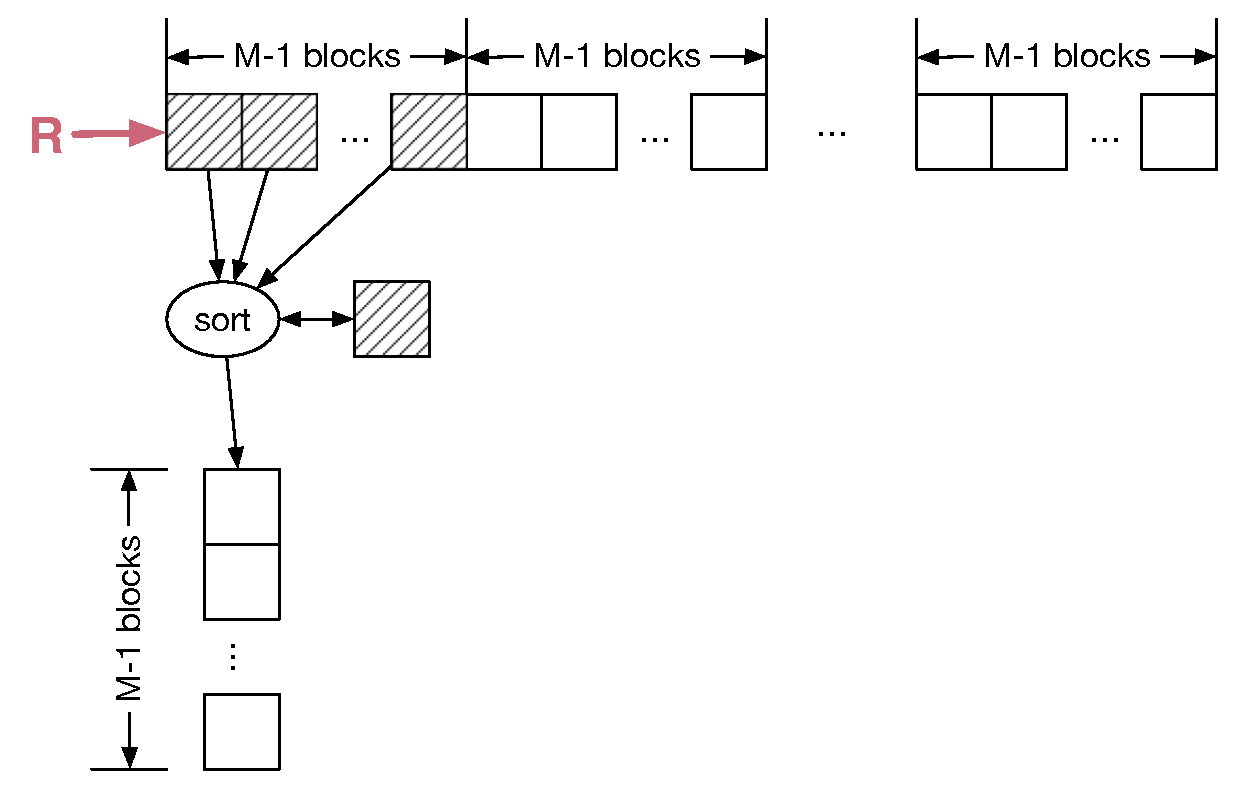
\includegraphics[width=0.75\textwidth]{figures/mergesort/step1.eps}};}
\onslide<2|handout:0>{\node at (0,0) {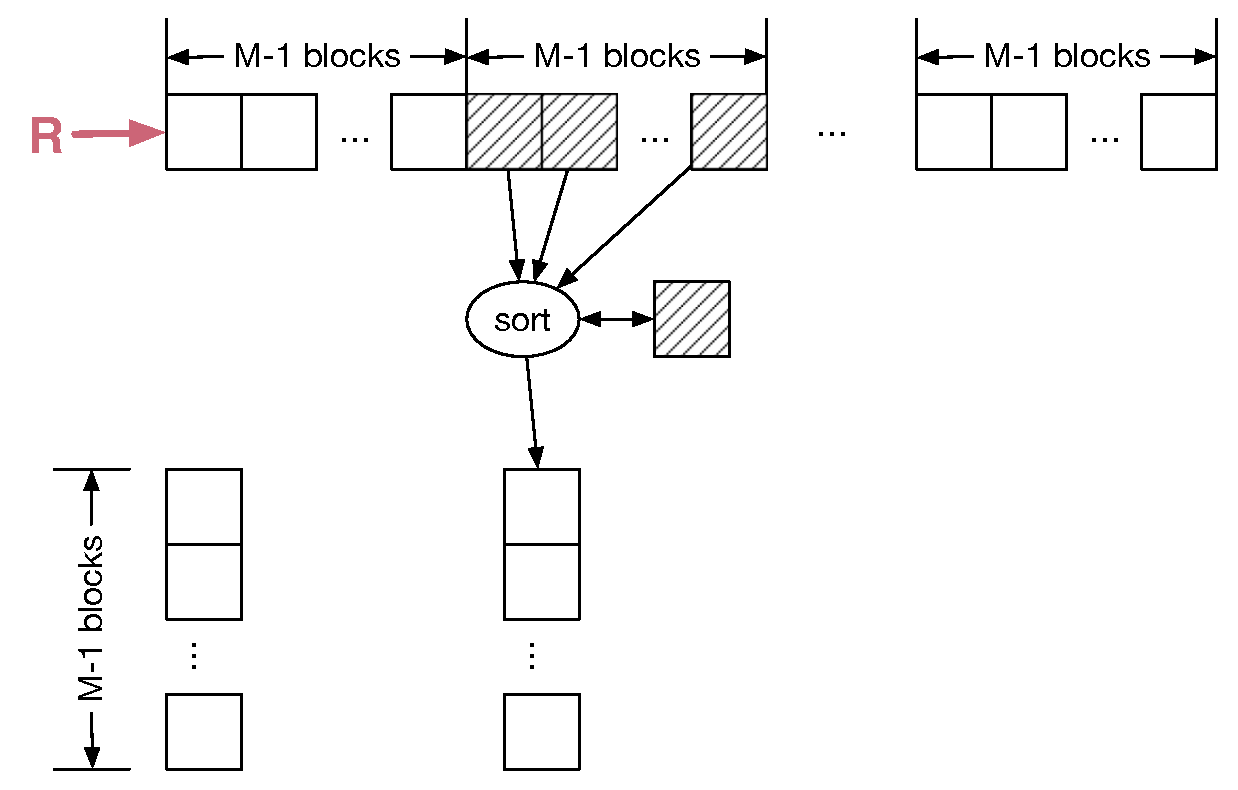
\includegraphics[width=0.75\textwidth]{figures/mergesort/step2.eps}};}
\onslide<3|handout:1>{\node at (0,0) {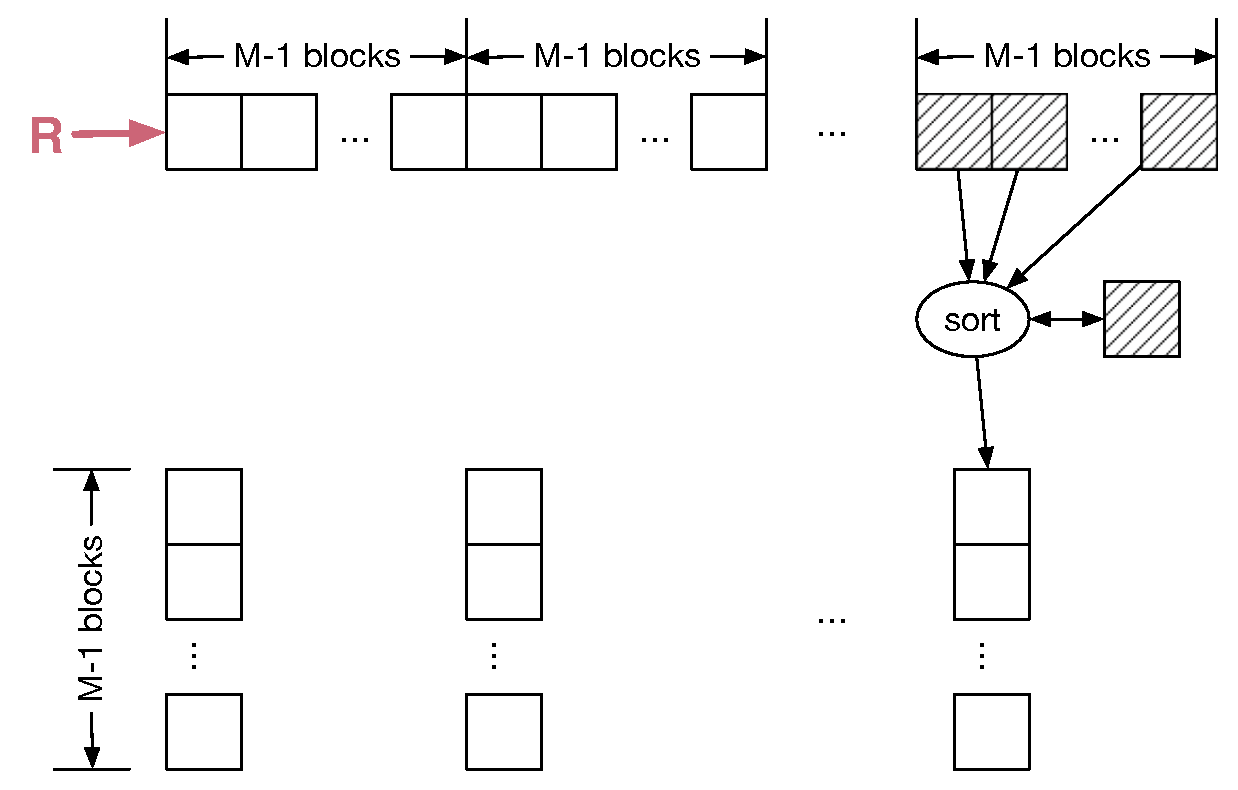
\includegraphics[width=0.75\textwidth]{figures/mergesort/step3.eps}};}
\end{tikzpicture}

\end{center}

\end{frame}

%
% --------------------------------------------------------------------------
%
\begin{frame}

\textbf{Step 2:} Merge the $N$ sorted chunks into a single sorted file. \alert{Case when $N\leq M-1$}:

\vskip2em

\begin{center}
\begin{tikzpicture}
\onslide<1|handout:0>{\node at (0,0) {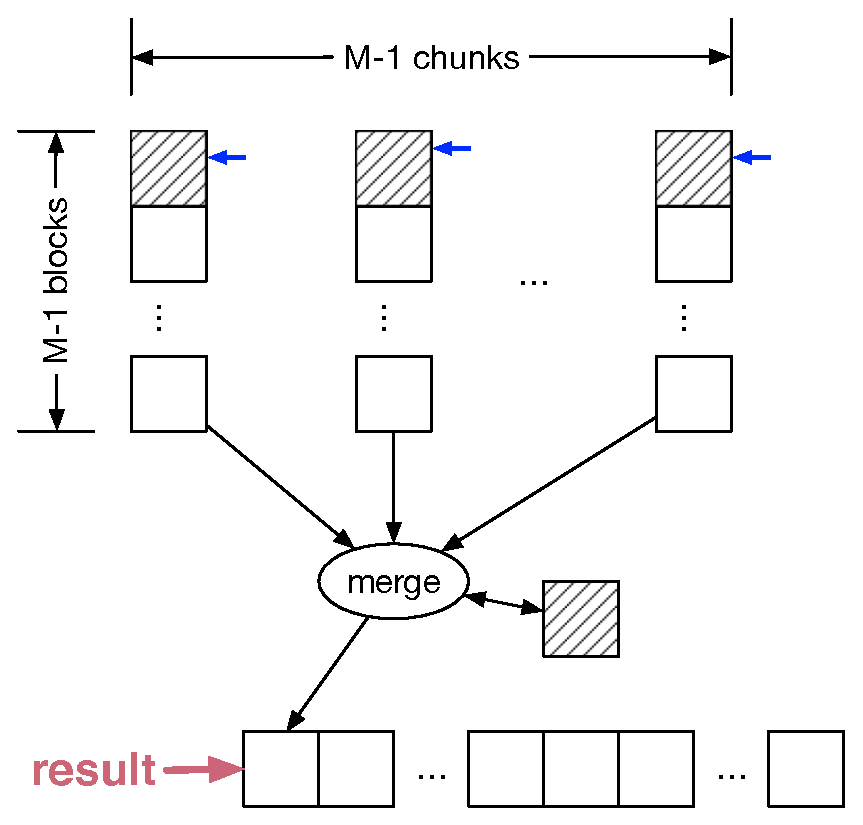
\includegraphics[width=0.5\textwidth]{figures/mergesort/step4.eps}};}
\onslide<2|handout:0>{\node at (0,0) {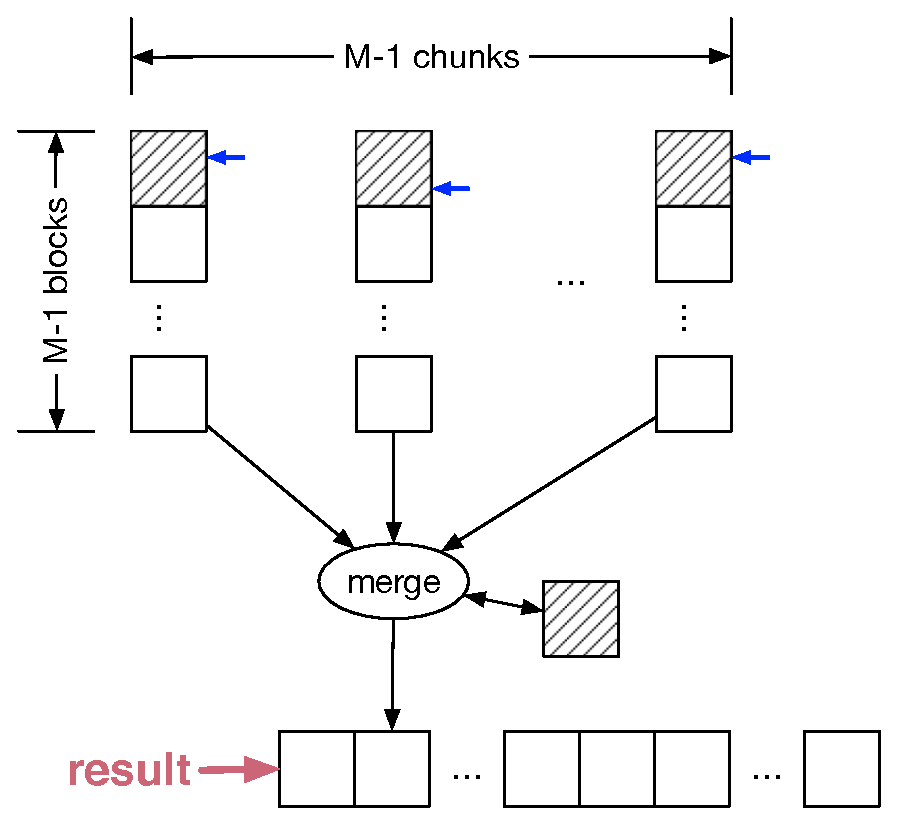
\includegraphics[width=0.5\textwidth]{figures/mergesort/step5.eps}};}
\onslide<3-|handout:1>{\node at (0,0) {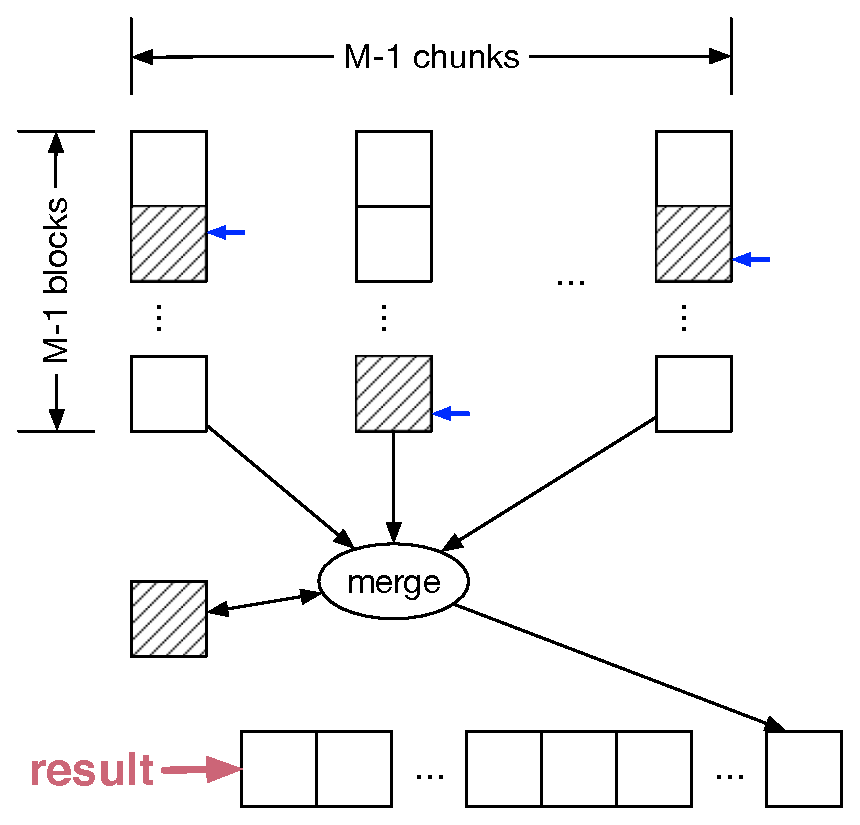
\includegraphics[width=0.5\textwidth]{figures/mergesort/step6.eps}};}
\end{tikzpicture}
\end{center}

\vskip1em

\onslide<4|handout:1>{When $N\leq M-1$ only one merge operation is needed.}

\end{frame}


%
% --------------------------------------------------------------------------
%
\begin{frame}

\textbf{Step 2 revisited} \alert{when $N > M-1$}:

\begin{center}
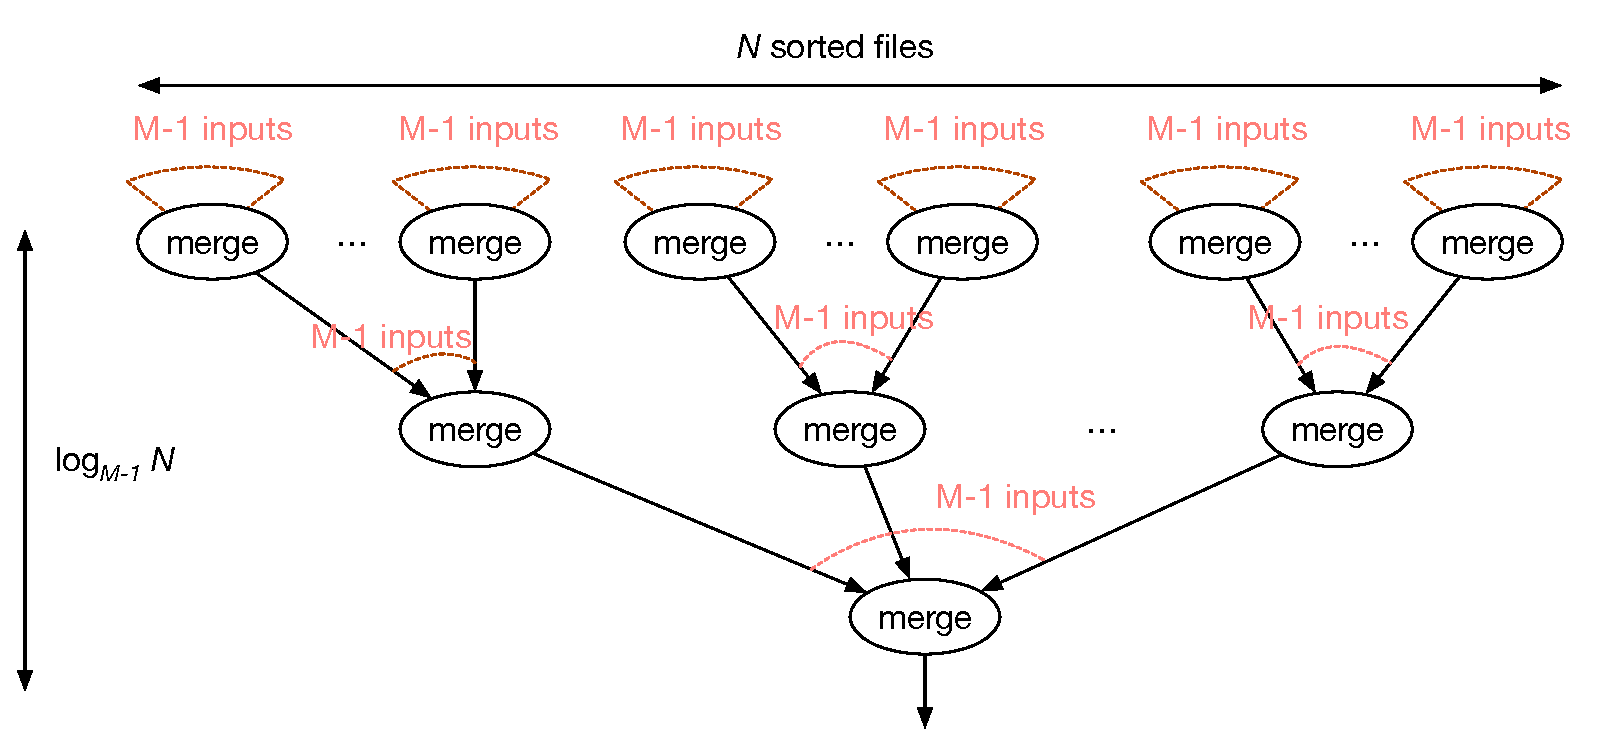
\includegraphics[width=0.85\textwidth]{figures/mergesort/merge_sort_part2_FULL}
\end{center}

This is like in-RAM mergesort, except that each merge steps has $M-1$ inputs \textbf{instead of} two.
\begin{itemize}[-,noitemsep,topsep=-0.5em]
\item The tree has $\ceil*{\log_{M-1}N}$ levels.
\item The entire table is read and written in each level, for a total I/O cost of \fbox{$O(|R|\ceil*{\log_{M-1}N})$}
\end{itemize}
\end{frame}

\begin{frame}

\vskip1em

\textbf{External multi-way mergesort}:\\
$M:$ buffers available; $|R|$: blocks to sort; $N=\ceil*{\frac{|R|}{M-1}}$: chunks.

\begin{itemize}[-]
\item \textbf{Sort phase:} load, sort and write each chunk.
\item \textbf{Merge phase:} start with $\mathit{pass} = 1$
\begin{enumerate}[(1)]
\item Merge the sorted chunks, $M-1$ at a time.
\item If the pass produced $2$ or more chunks, increment $\mathit{pass}$ and repeat step (1).
\end{enumerate}
\end{itemize}

\vskip1em

\begin{block}{How much I/O in total? }

In \blue{each pass} on the file we \alert{read and write} the same amount of data (i.e., the size of the file itself):
\begin{itemize}[-,noitemsep,topsep=-0.5em]
\item Sort phase: $2\cdot |R|$
\item Merge phase: $2 \cdot \ceil*{\log_{M-1}N}|R|$
\end{itemize}

\end{block}
\end{frame}

%
% --------------------------------------------------------------------------
%
\begin{frame}[fragile]

\textbf{Example:} sorting relation \lstinline[style=SQL]{Member(name, class)} on \lstinline[style=SQL]!class! with $M=3$.

\vskip2em

\begin{center}
\begin{tikzpicture}
\onslide<1|handout:0>{\node at (0,0) {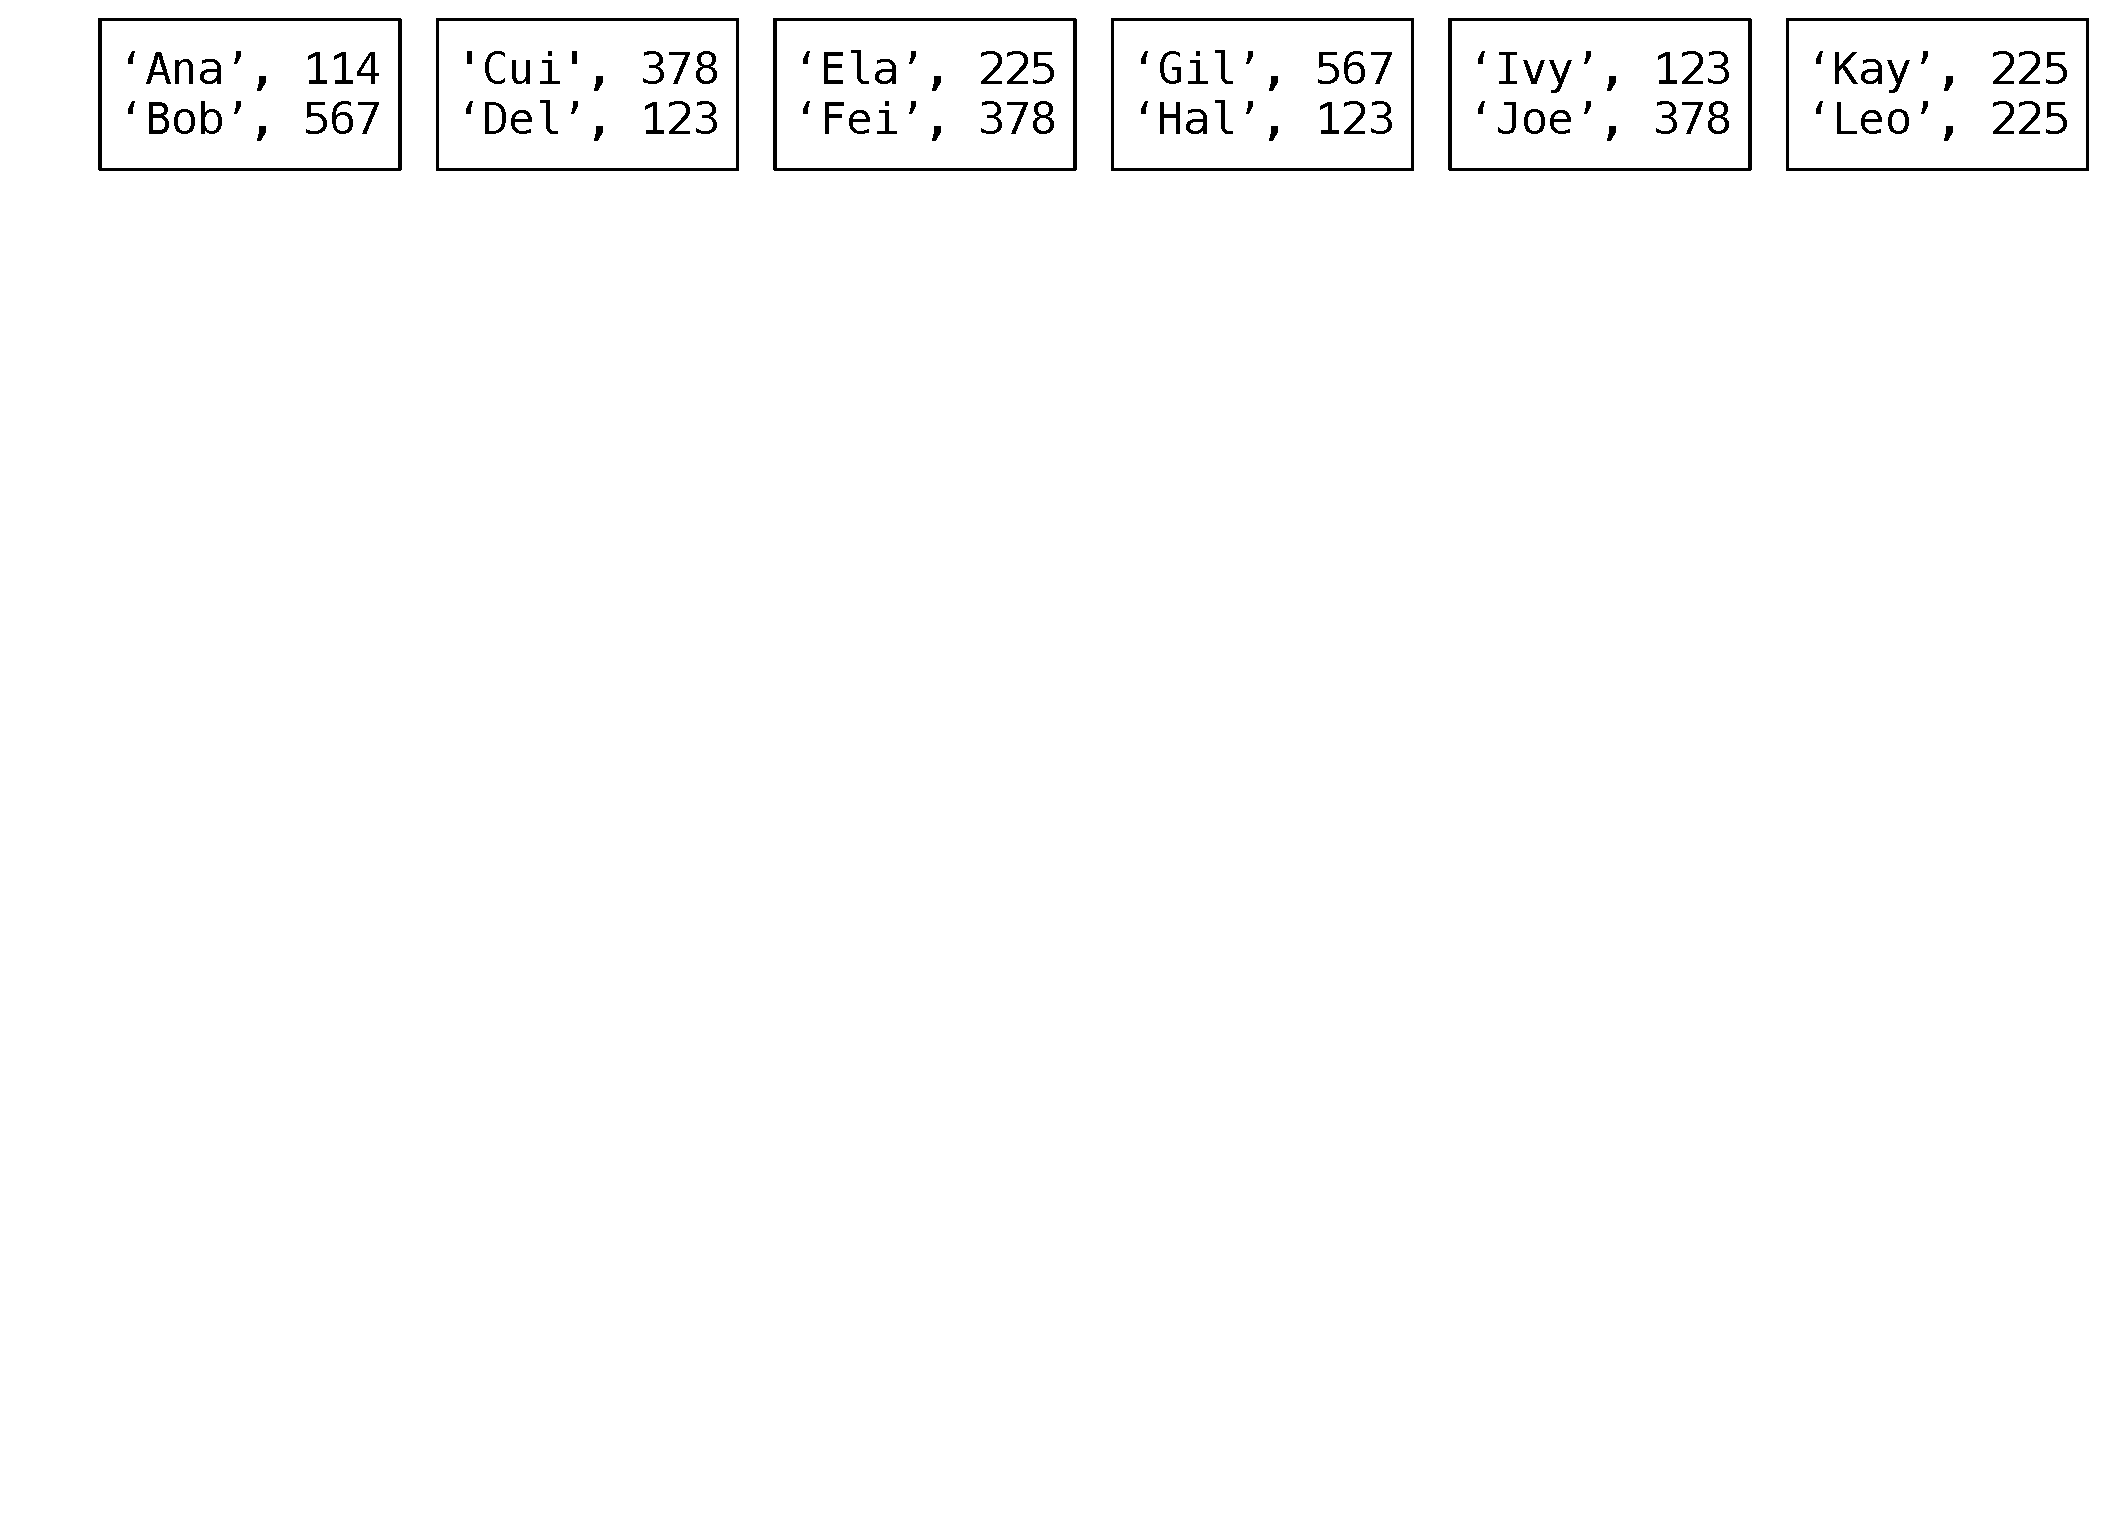
\includegraphics[width=0.9\textwidth]{figures/mergesort_example/step1.eps}};}
\onslide<2|handout:0>{\node at (0,0) {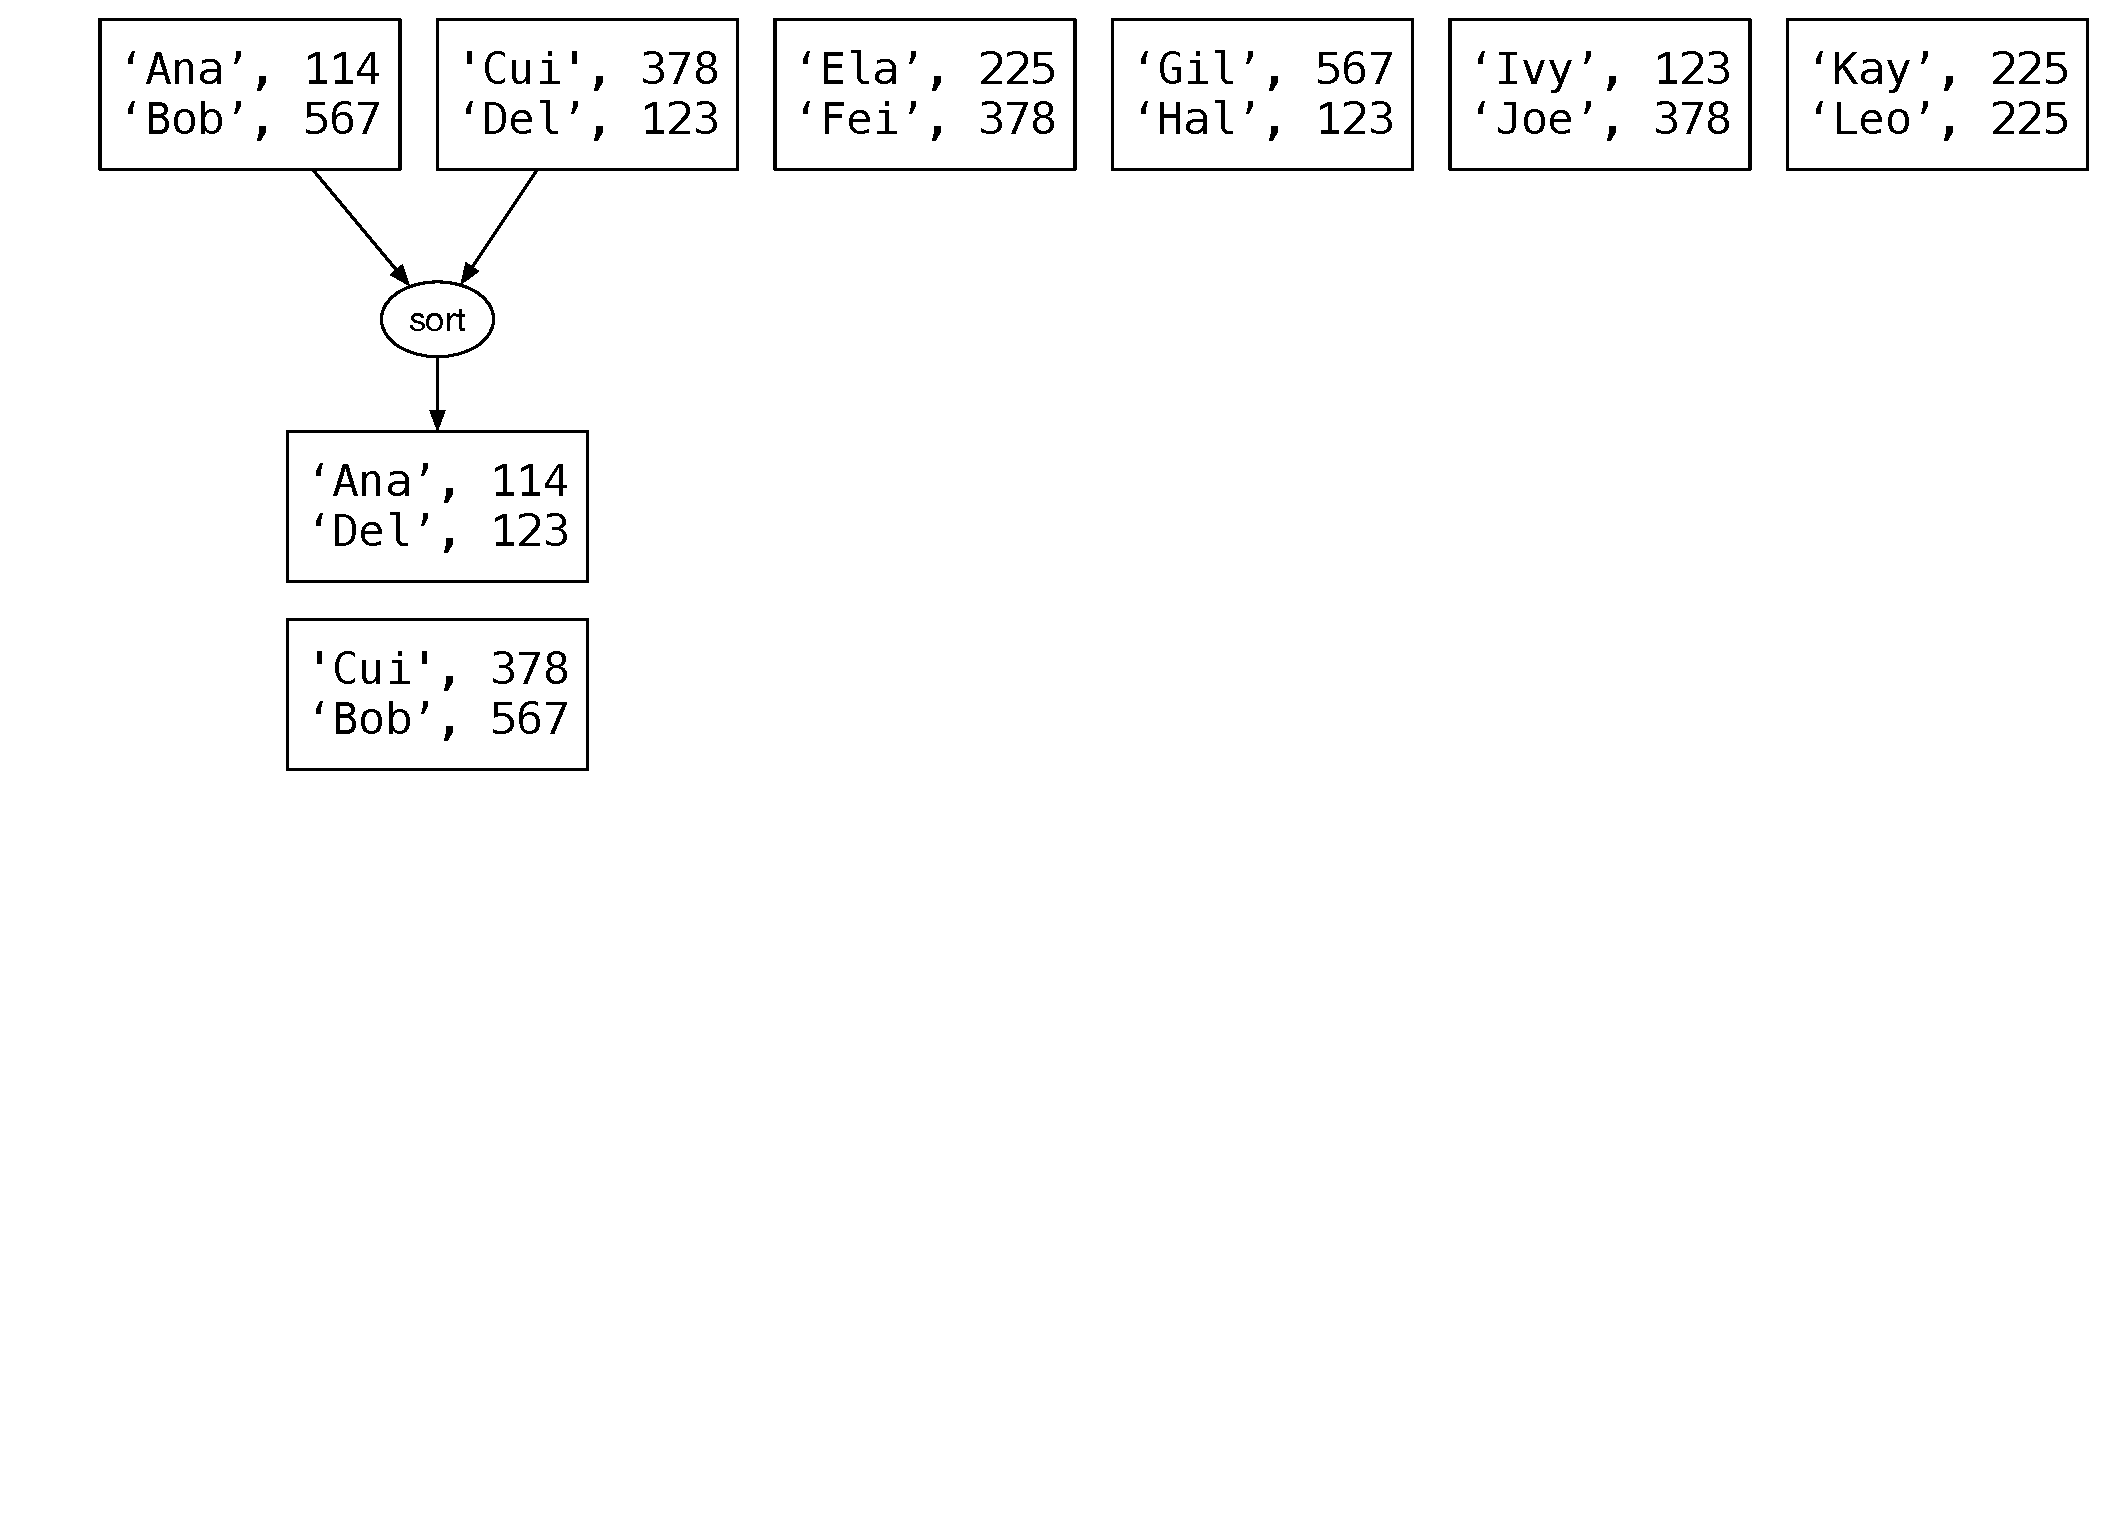
\includegraphics[width=0.9\textwidth]{figures/mergesort_example/step2.eps}};}
\onslide<3|handout:0>{\node at (0,0) {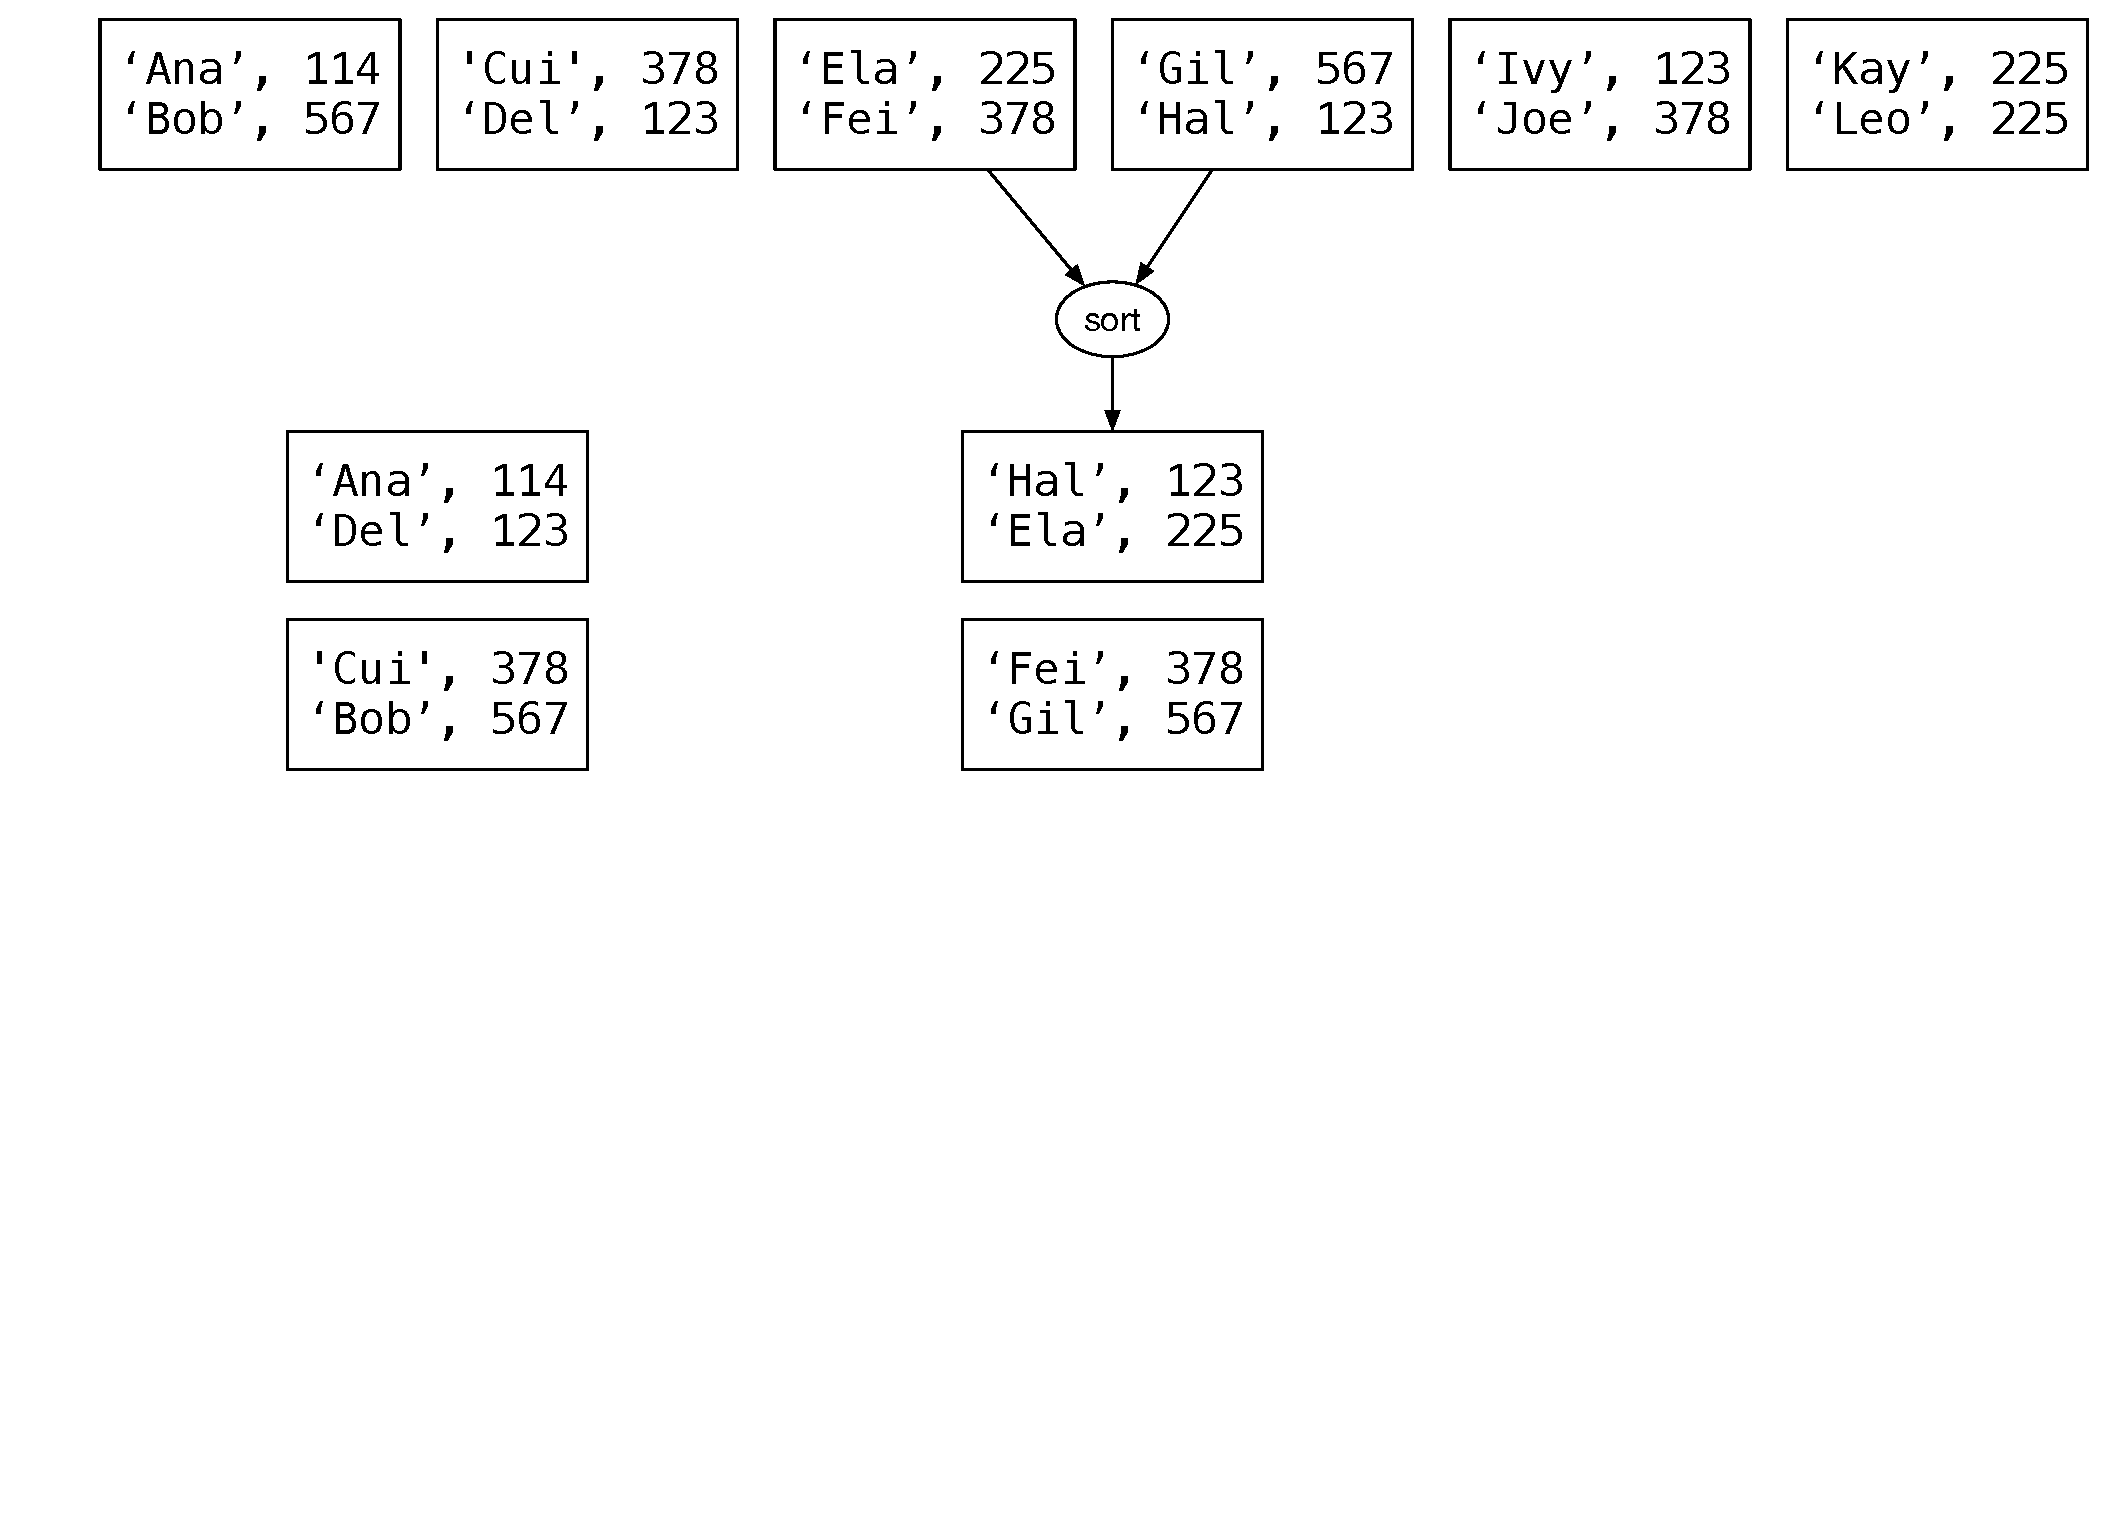
\includegraphics[width=0.9\textwidth]{figures/mergesort_example/step3.eps}};}
\onslide<4|handout:0>{\node at (0,0) {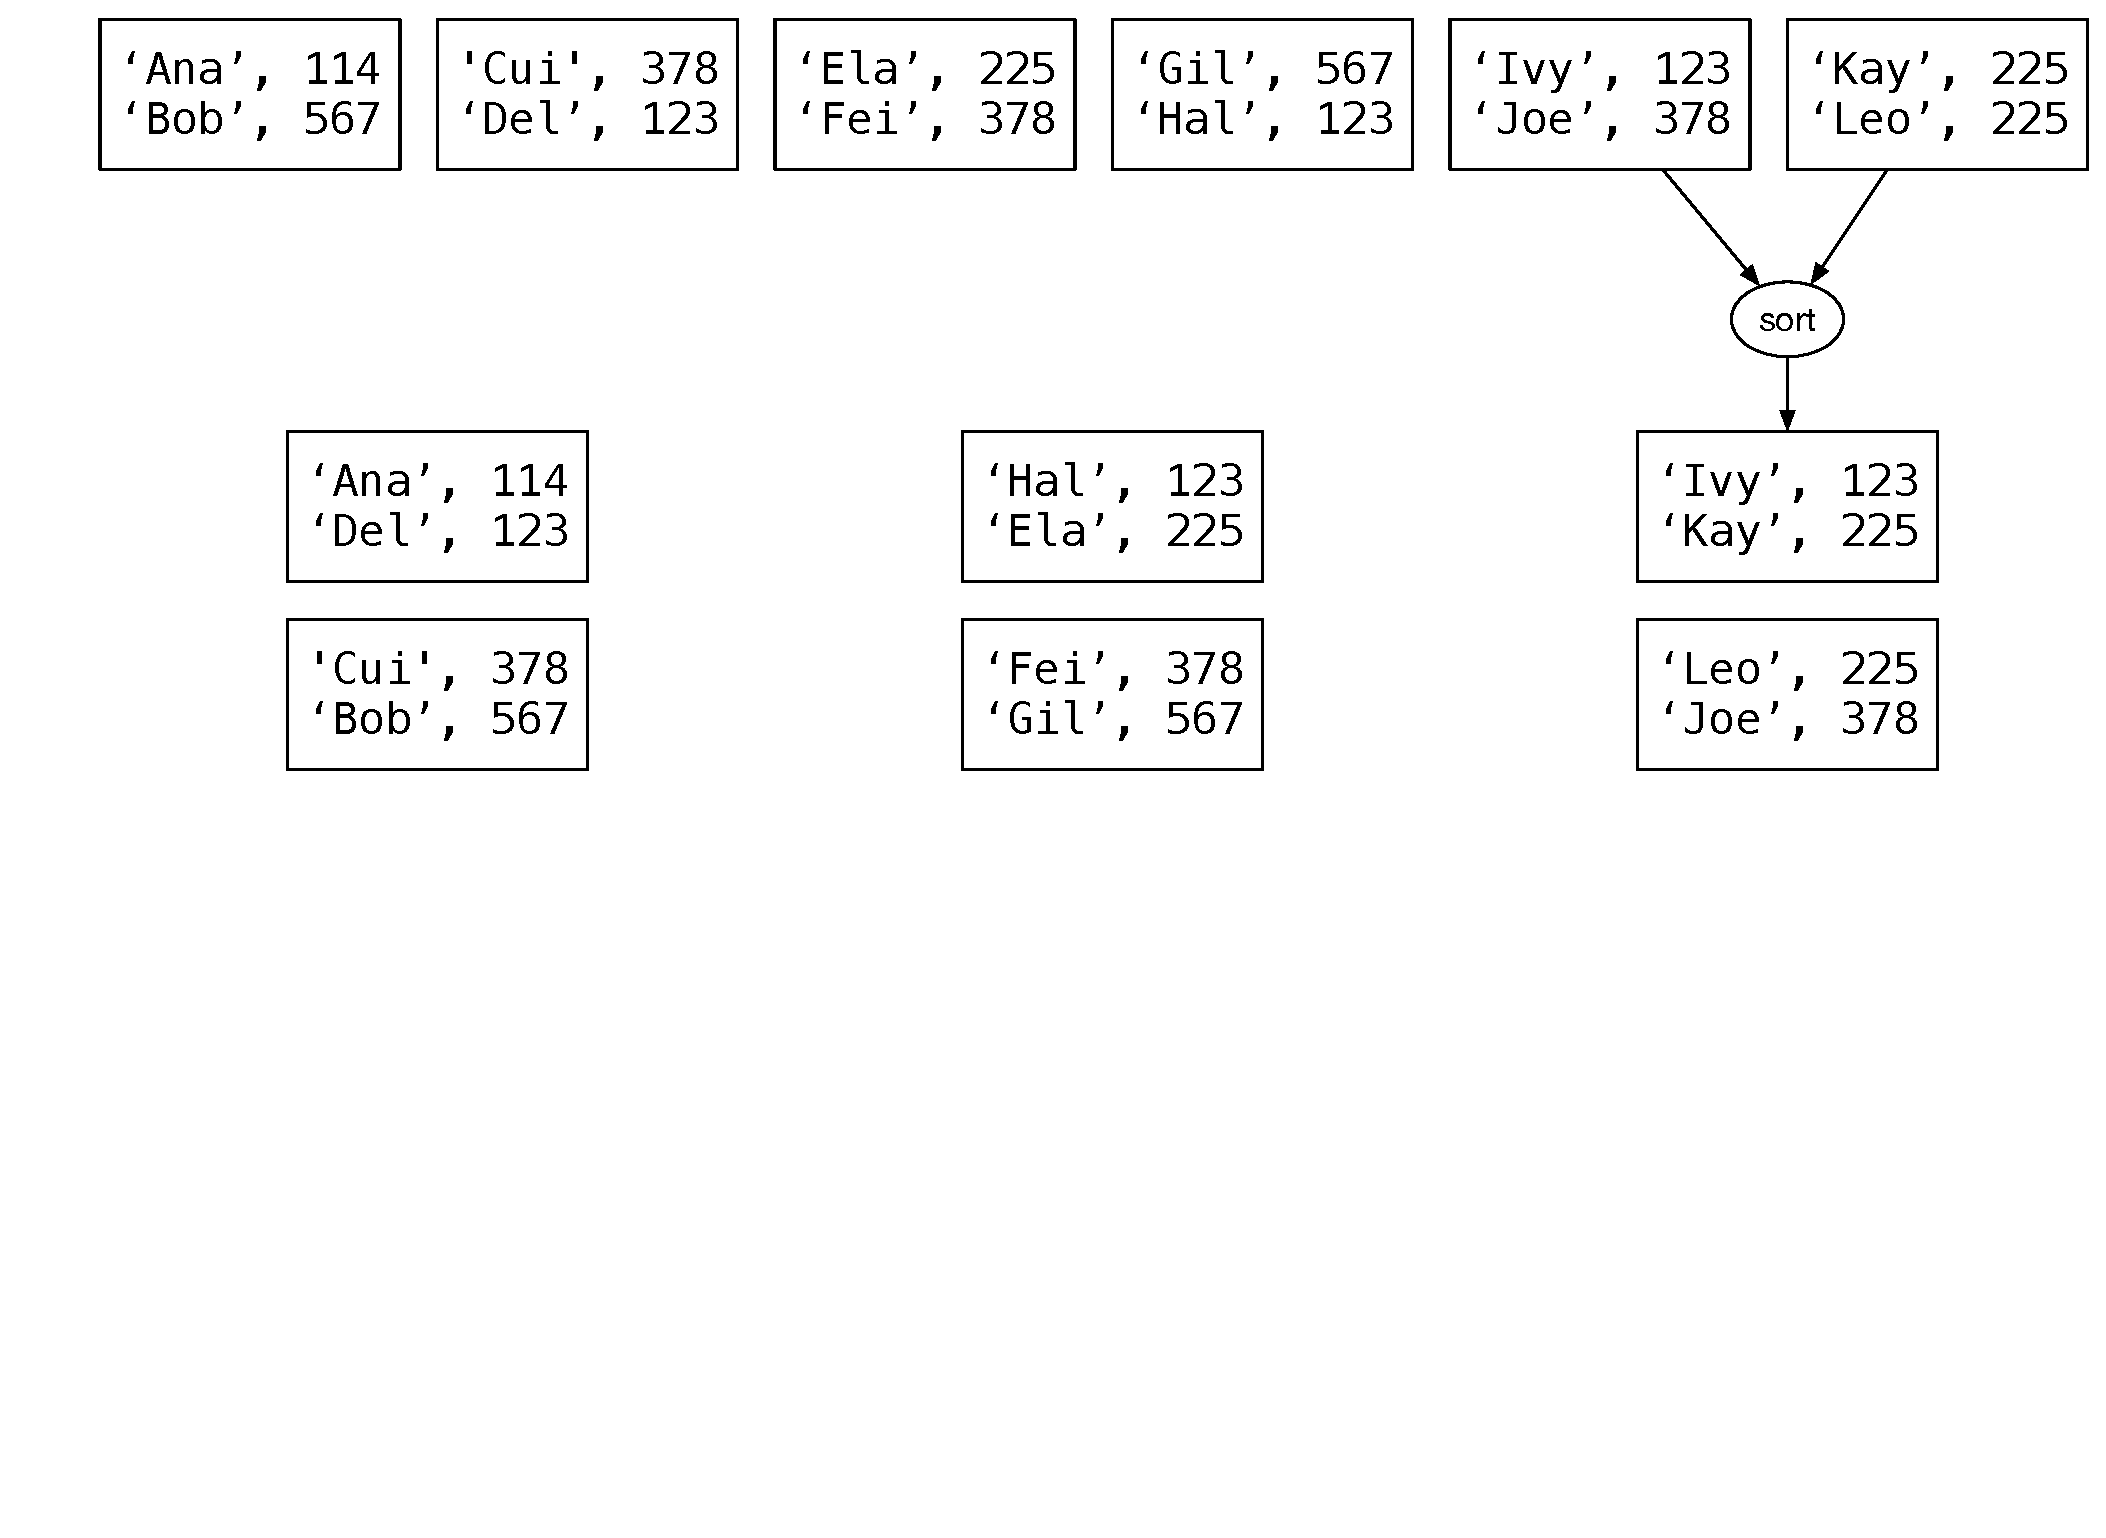
\includegraphics[width=0.9\textwidth]{figures/mergesort_example/step4.eps}};}
\onslide<5|handout:0>{\node at (0,0) {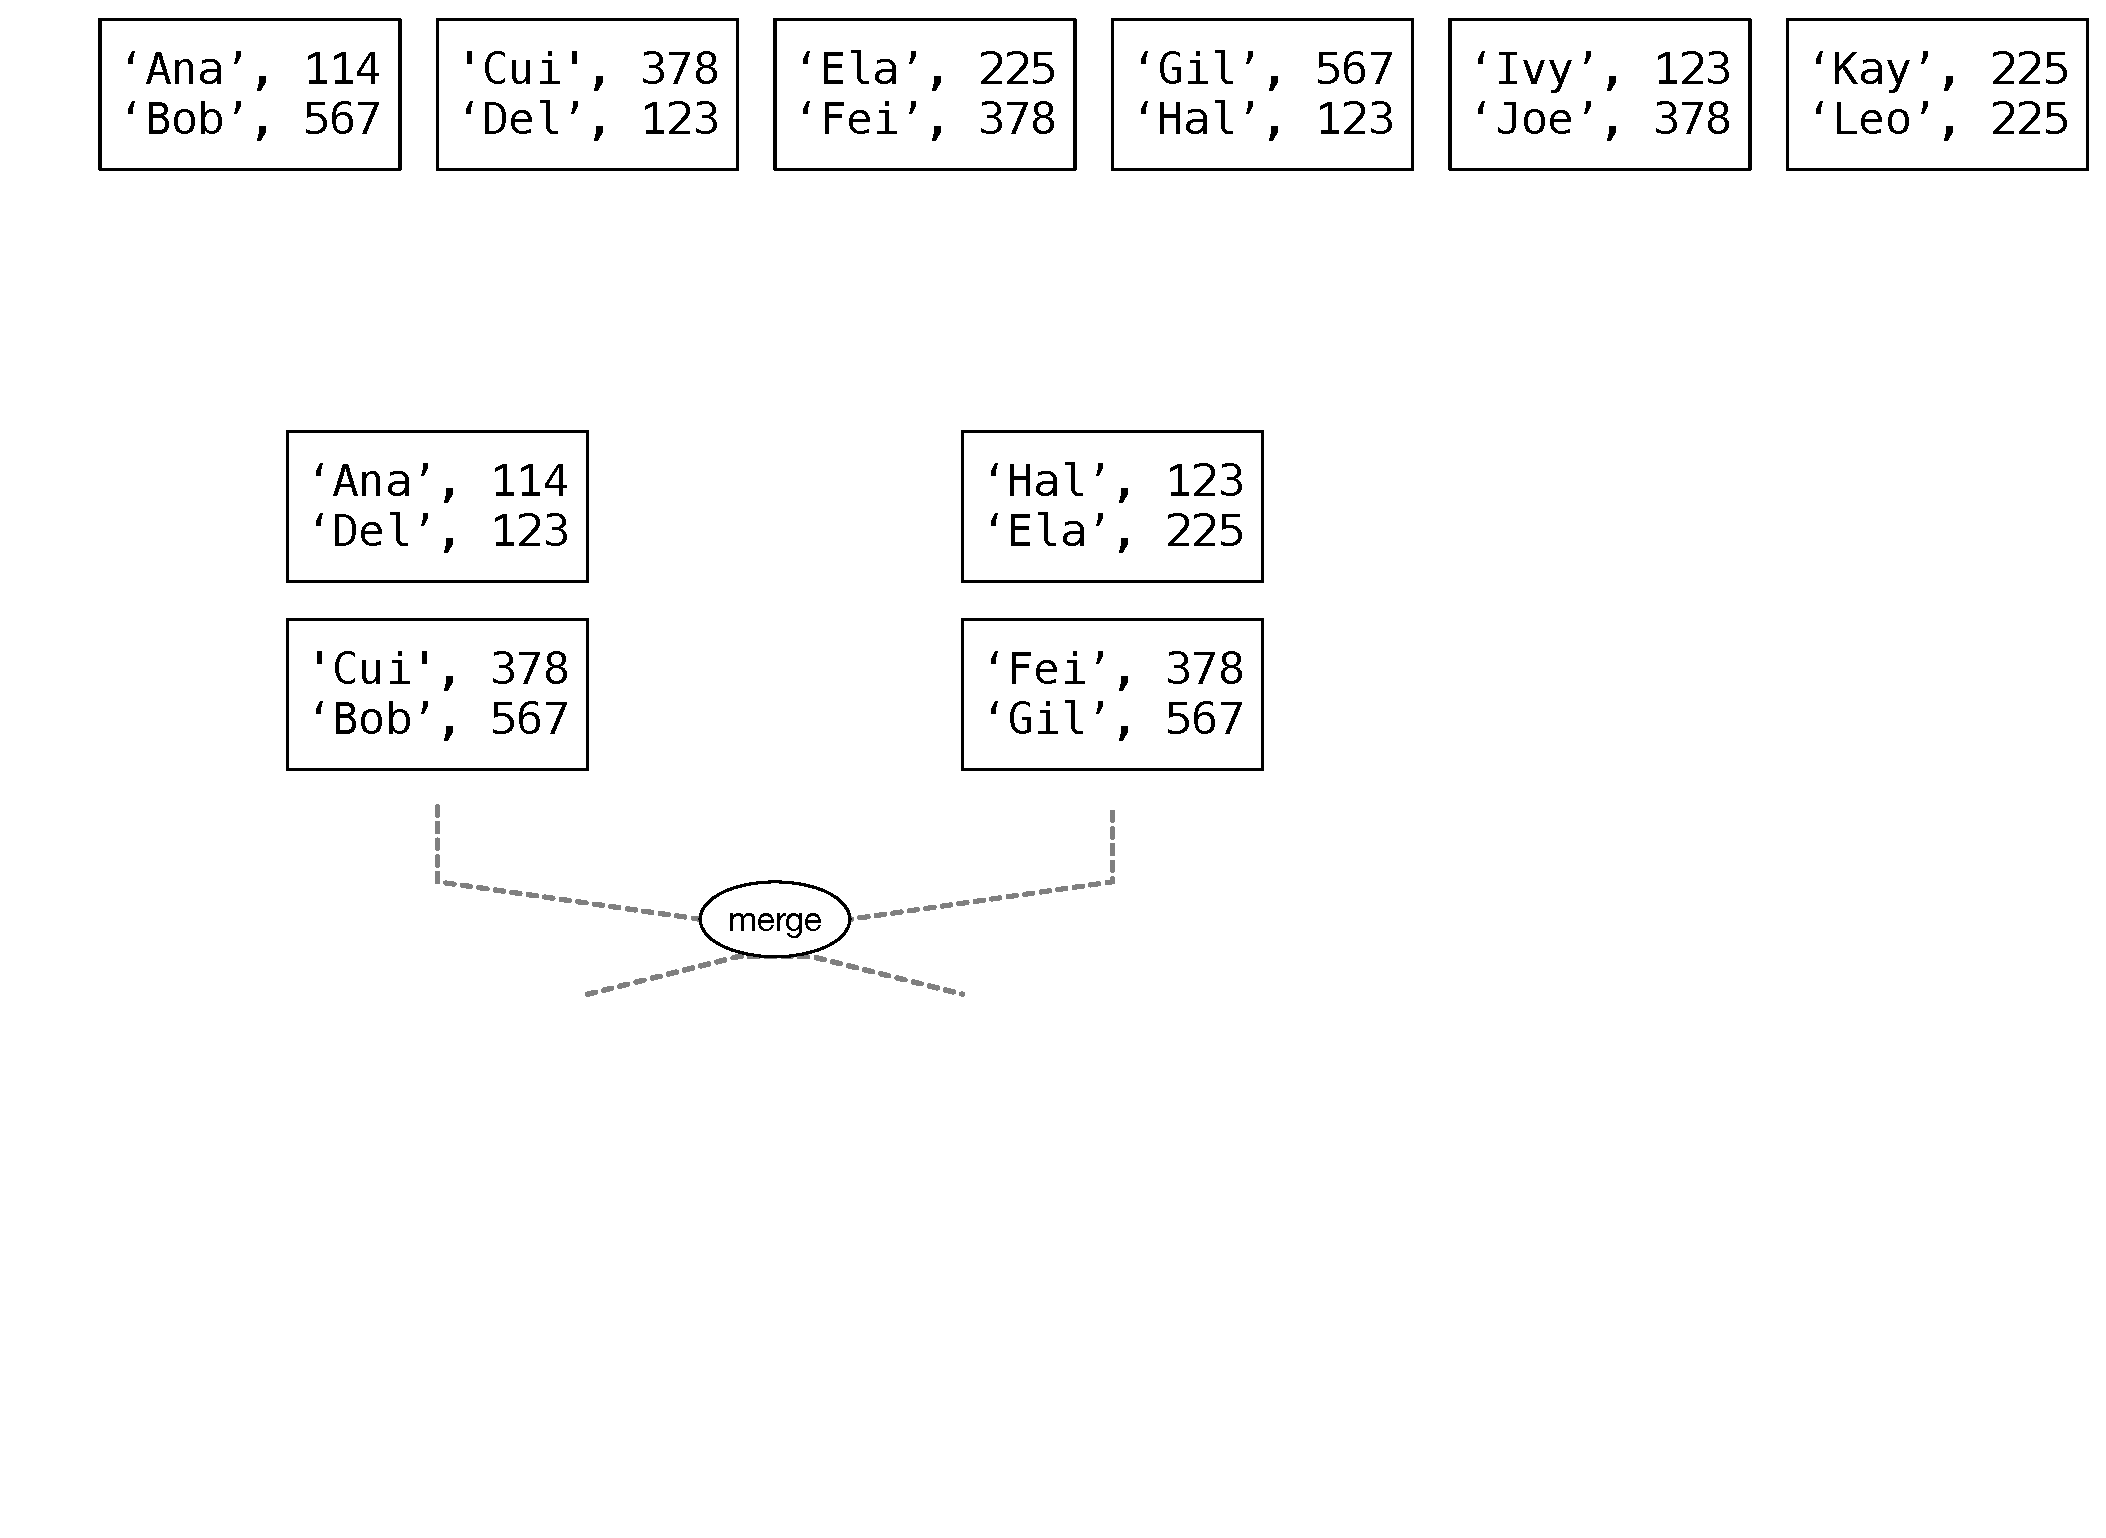
\includegraphics[width=0.9\textwidth]{figures/mergesort_example/step5.eps}};}
\onslide<6|handout:0>{\node at (0,0) {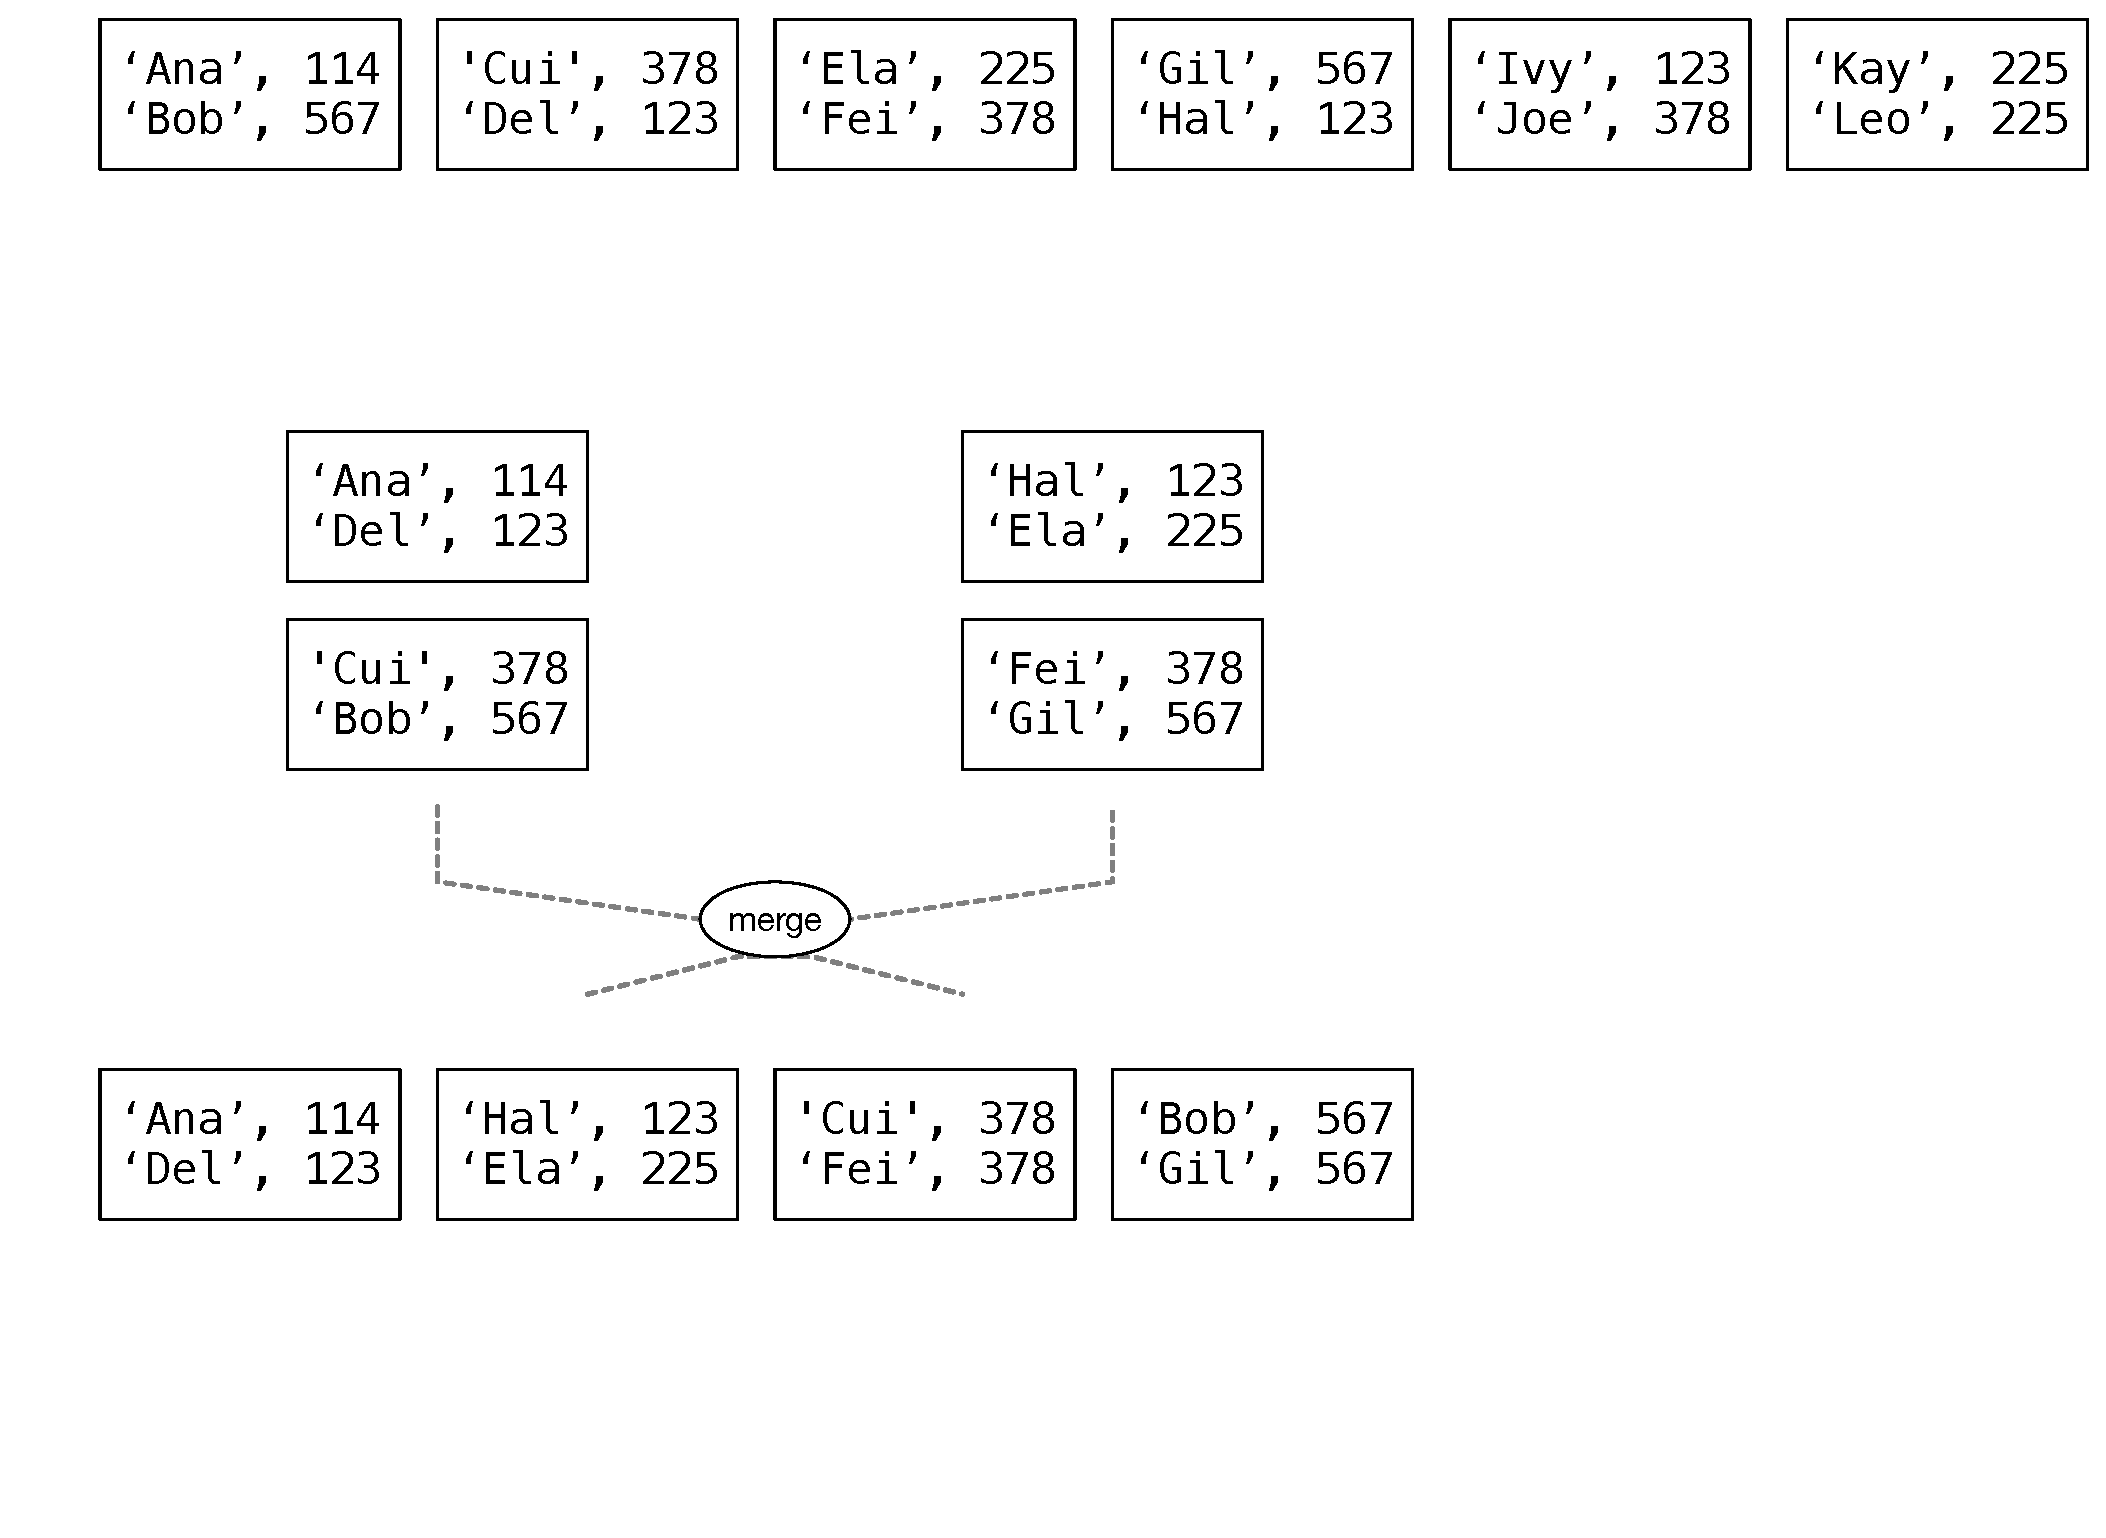
\includegraphics[width=0.9\textwidth]{figures/mergesort_example/step6.eps}};}
\onslide<7|handout:0>{\node at (0,0) {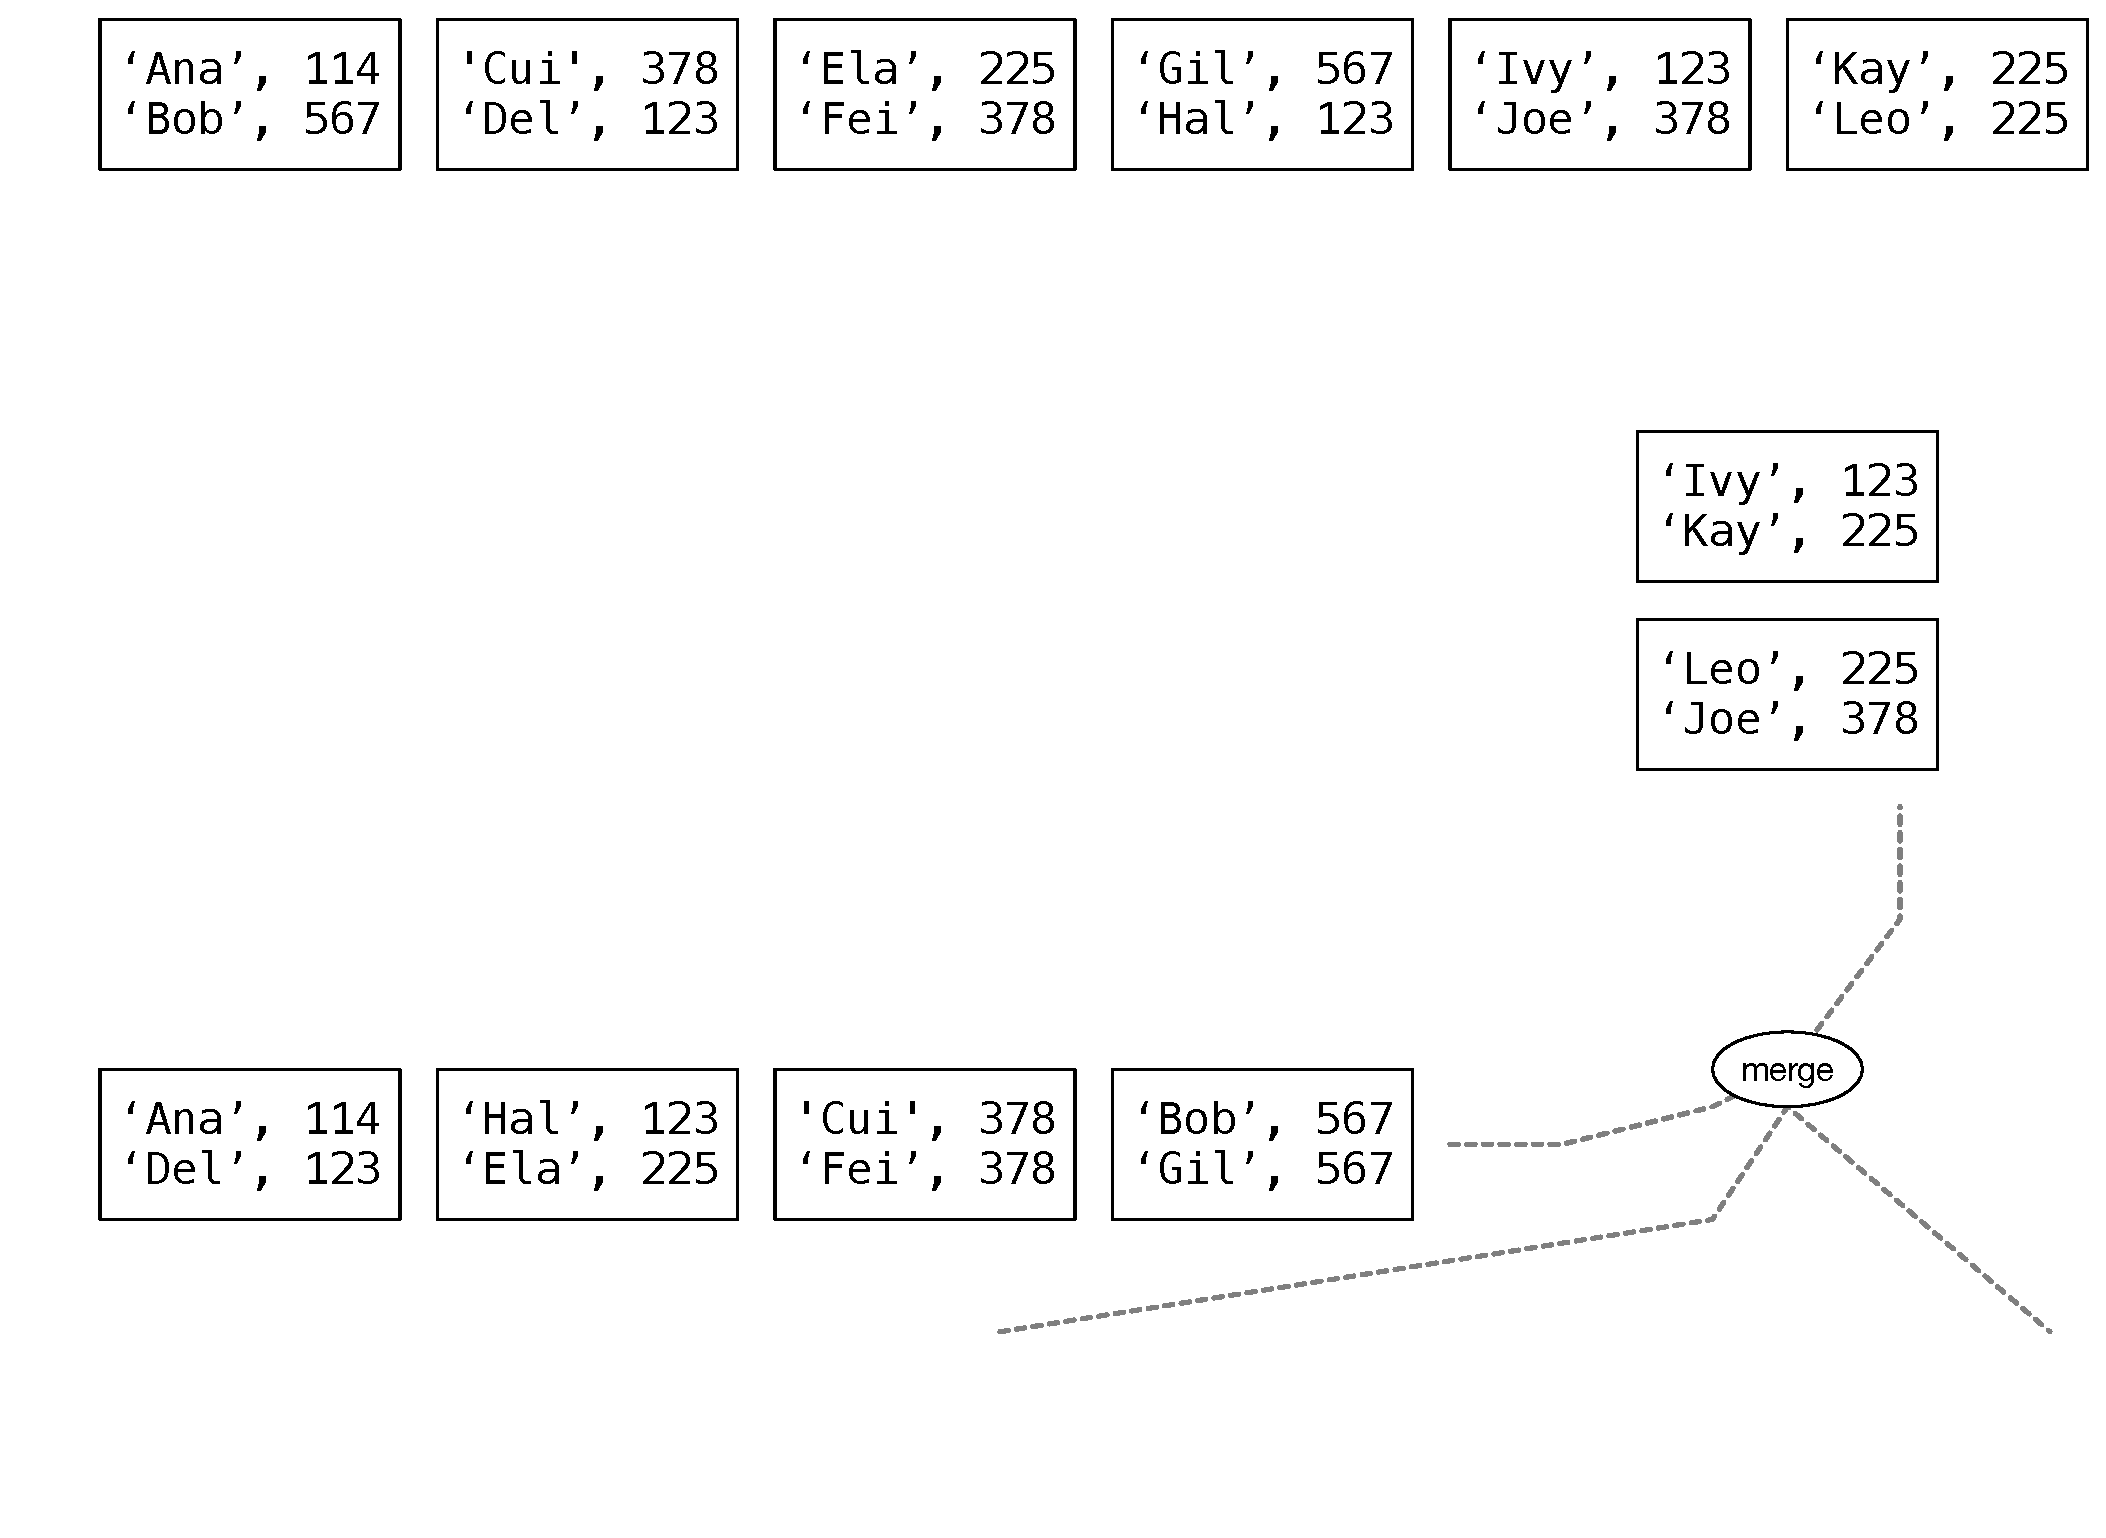
\includegraphics[width=0.9\textwidth]{figures/mergesort_example/step7.eps}};}
\onslide<8|handout:0>{\node at (0,0) {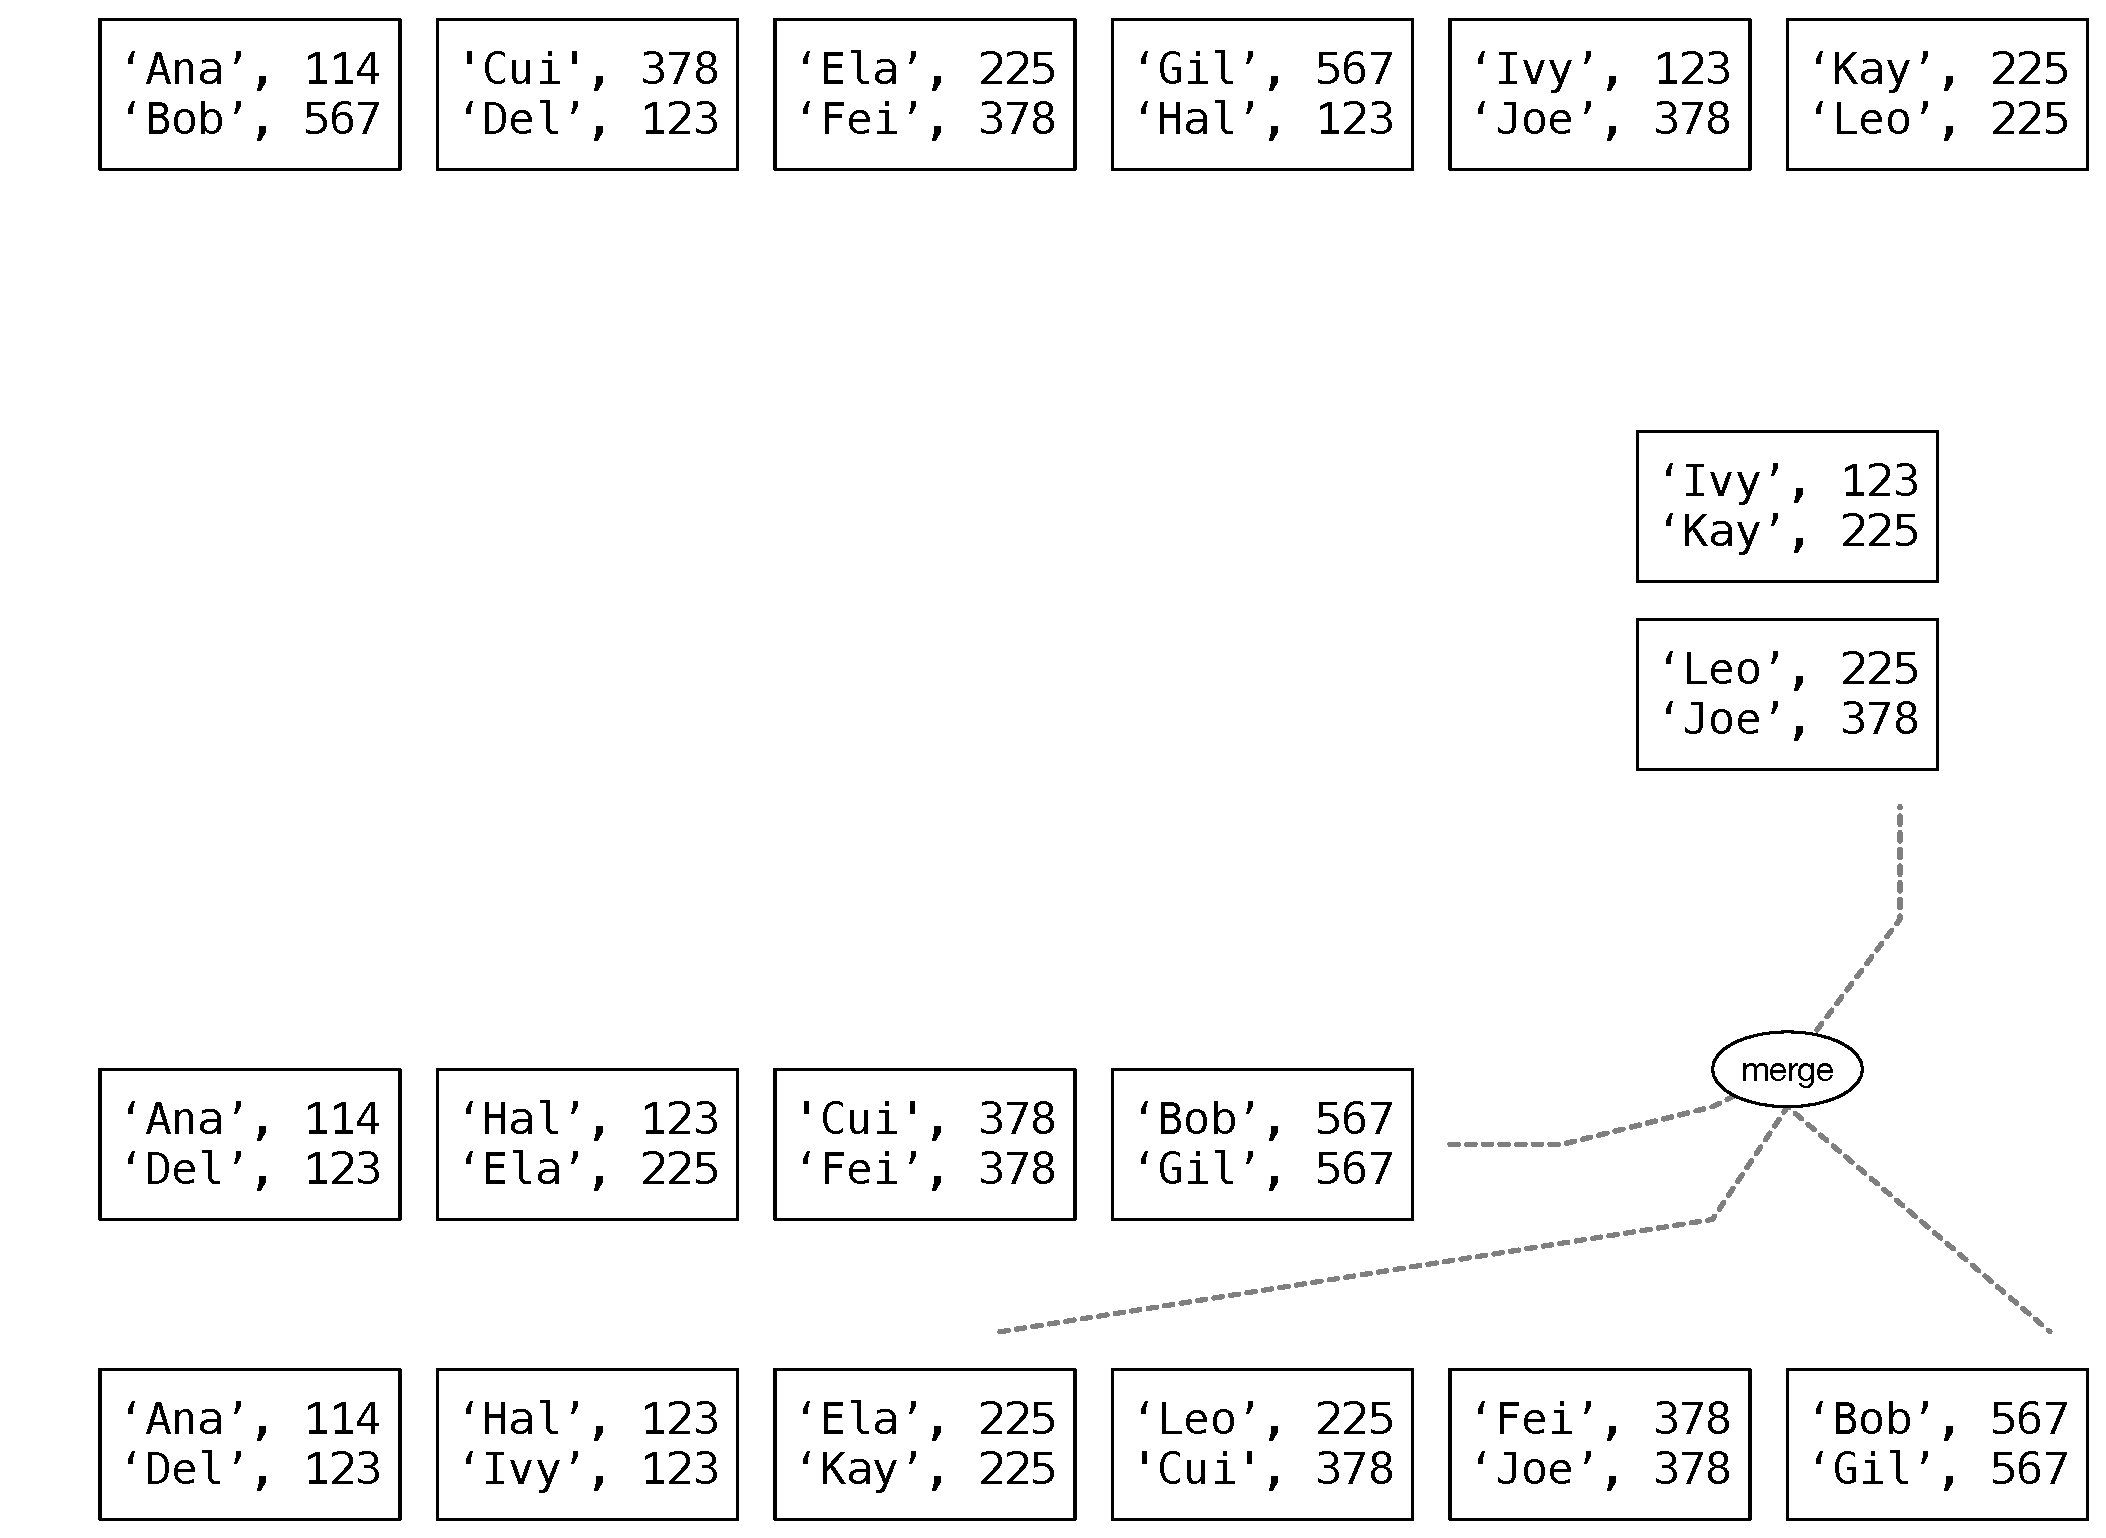
\includegraphics[width=0.9\textwidth]{figures/mergesort_example/step8.eps}};}
\onslide<9|handout:1>{\node at (0,0) {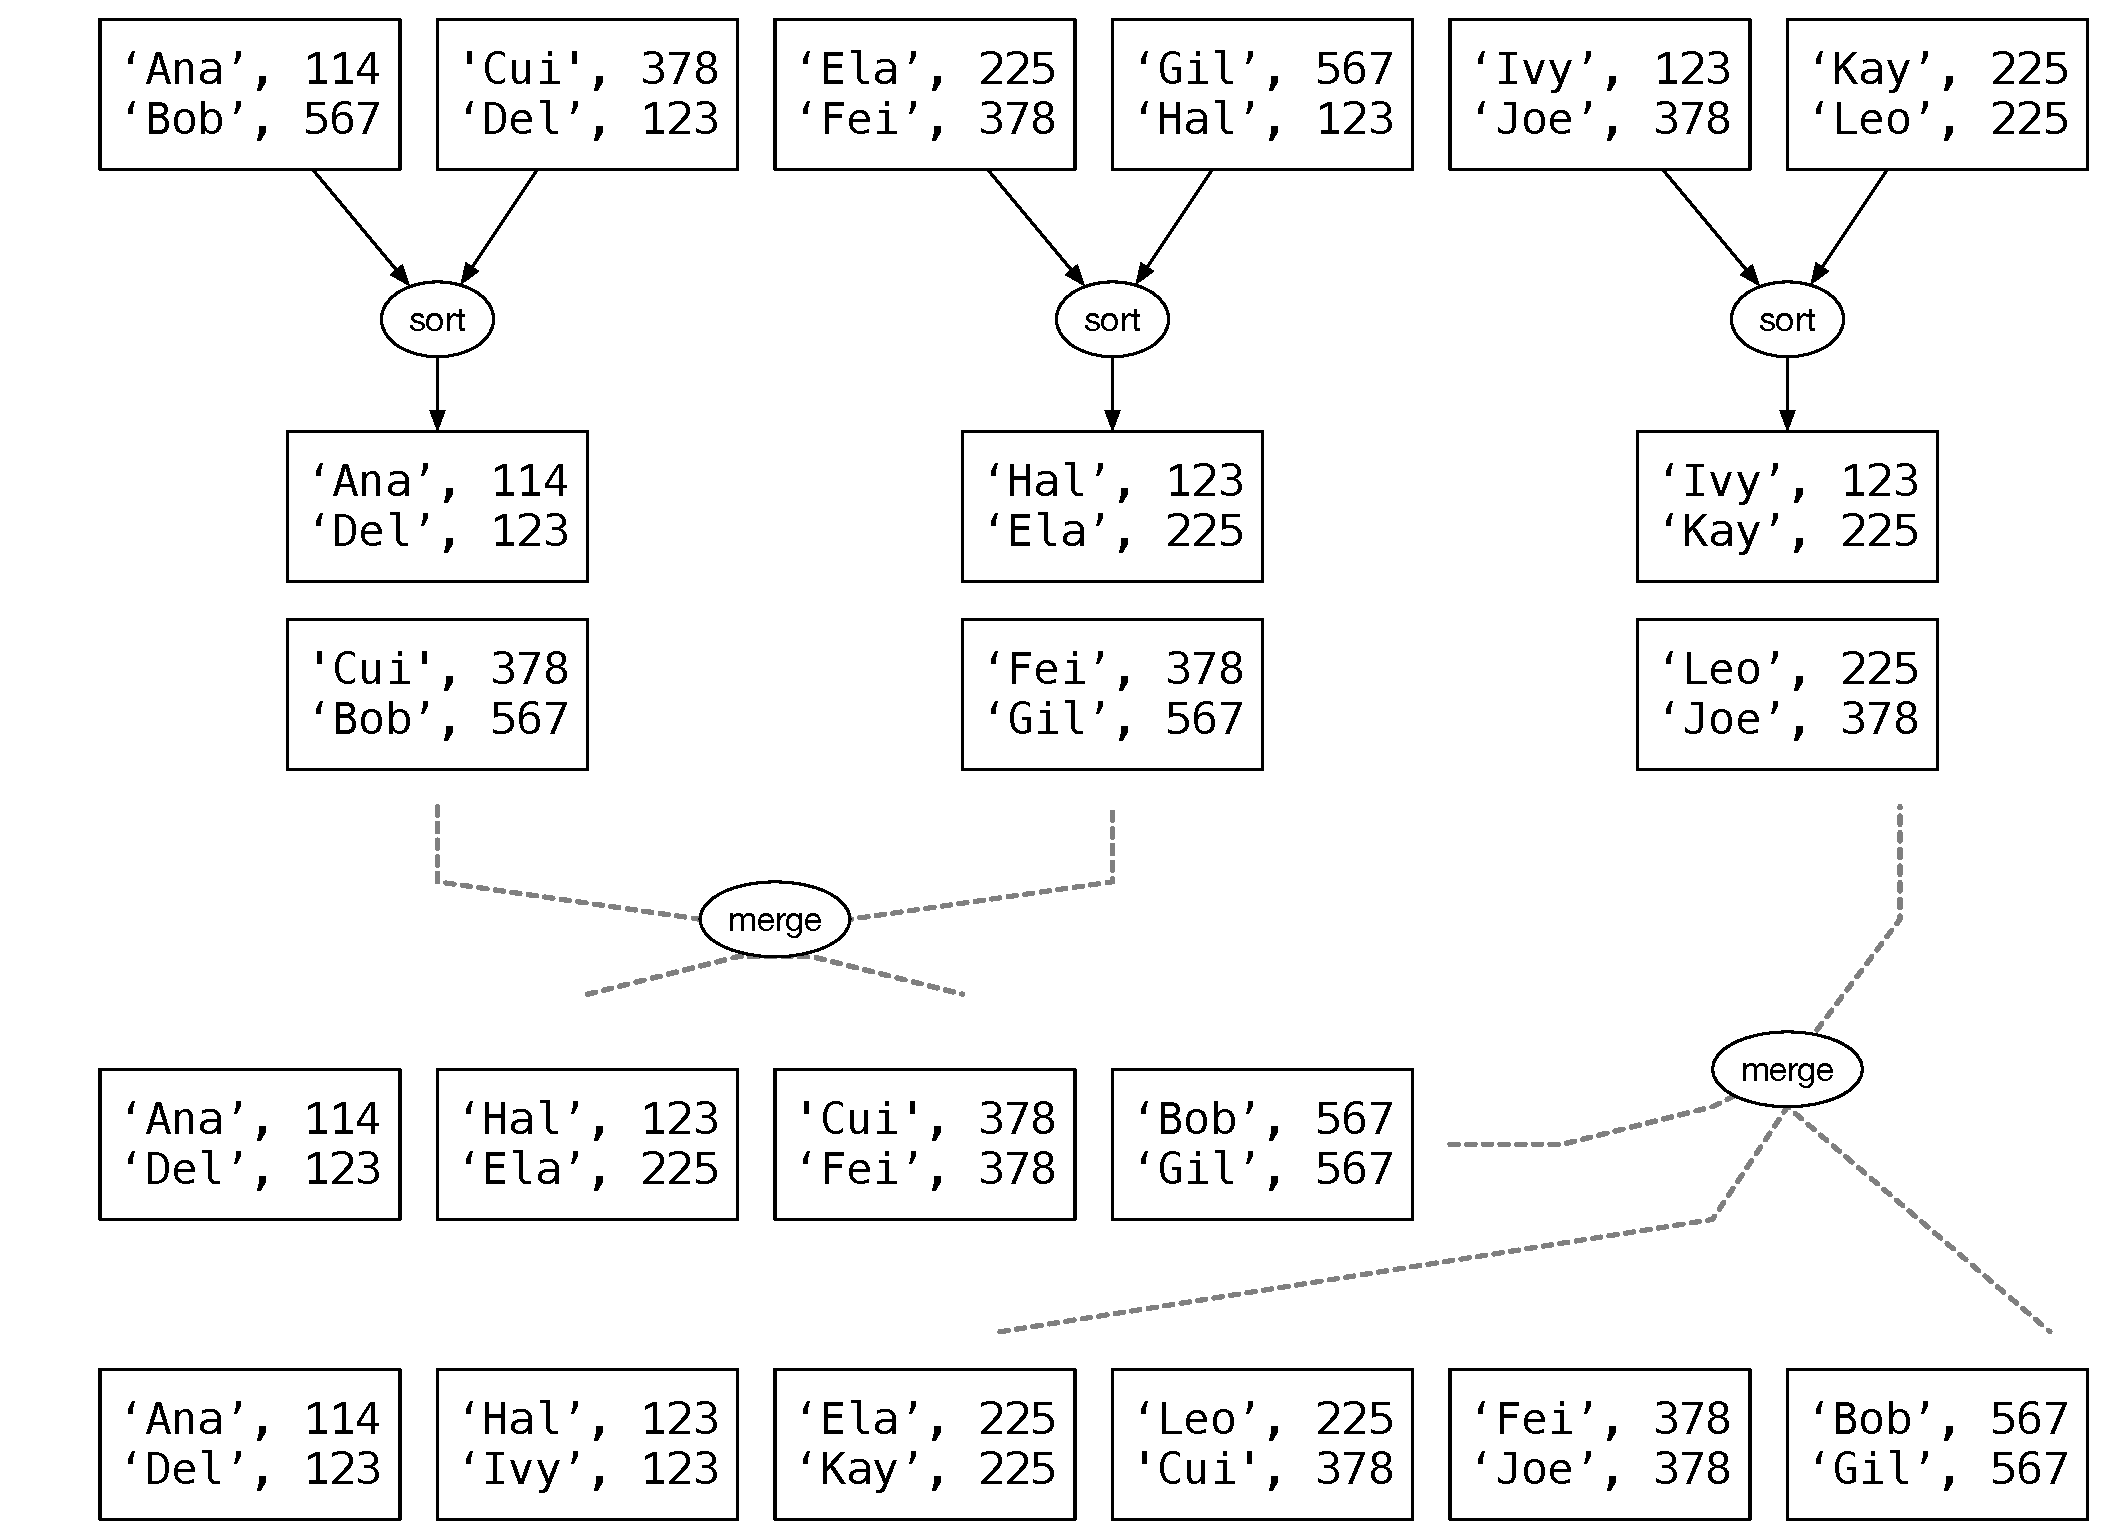
\includegraphics[width=0.9\textwidth]{figures/mergesort_example/final.eps}};}
\end{tikzpicture}
\end{center}

\end{frame}

%
% --------------------------------------------------------------------------
%
\begin{frame}{Sort-based Equality Join $R.a = S.b$}
\label{sort_based_equality_join_idea}

\begin{enumerate}[label=(\arabic*)]
\item Make a sorted copy of $R$ (on \lstinline{R.a}) and another of $S$ (on \lstinline{S.b}) using the external merge-sort algorithm.
\item Scan the two sorted relations looking for tuples that match:
\begin{itemize}%[label=(\roman*)]
\item[$t_{R}$] : current tuple of $R$
\item[$t_{S1}$] : first tuple in $S$ such that $t_R.a = t_{S1}.b$
\item[$t_{S2}$] : current tuple in $S$ such that $t_R.a = t_{S2}.b$
\end{itemize}
\end{enumerate}

\vskip2em

\begin{center}
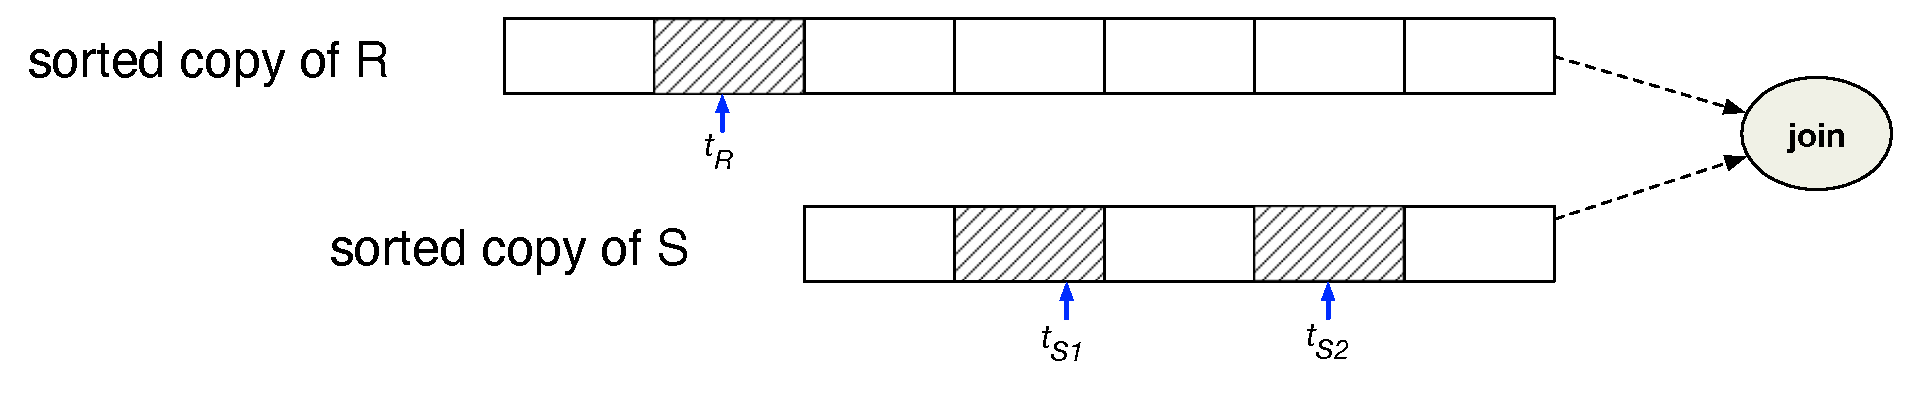
\includegraphics[width=\textwidth]{figures/sort_based_join}
\end{center}
\end{frame}

%
% --------------------------------------------------------------------------
%
\begin{frame}[fragile]

\textbf{Example:} \lstinline[style=SQL]!SELECT name, time FROM Member JOIN Schedule!

\vskip2em

\begin{center}
\begin{tikzpicture}
\node at (-1.05,4) {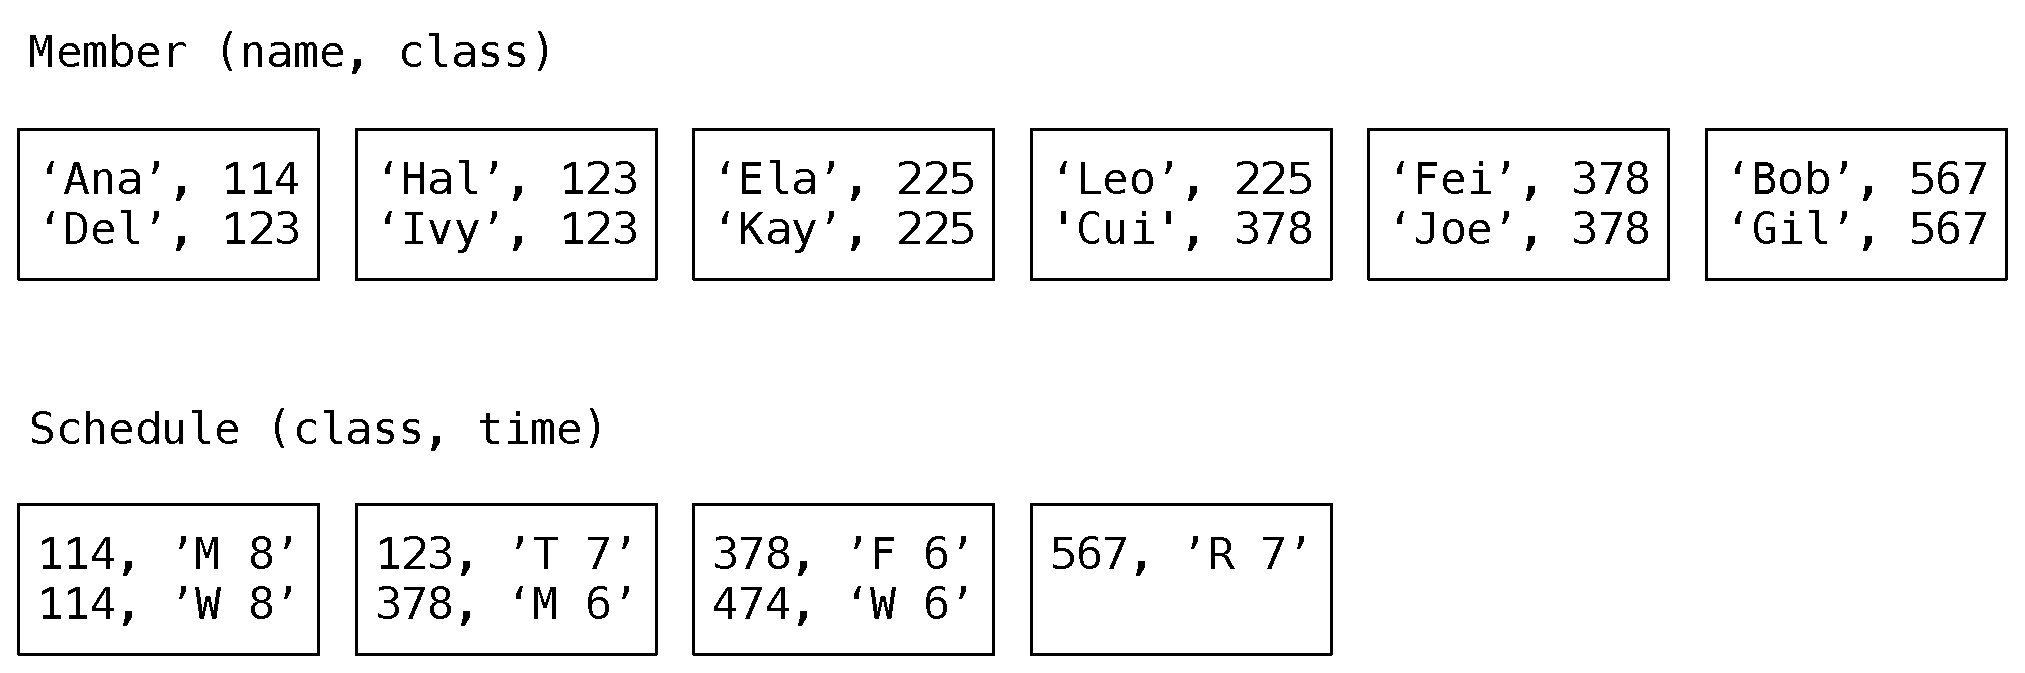
\includegraphics[width=0.85\textwidth]{figures/sort_join/sorted_tables.eps}};
\onslide<1|handout:0>{\node at (0,0) {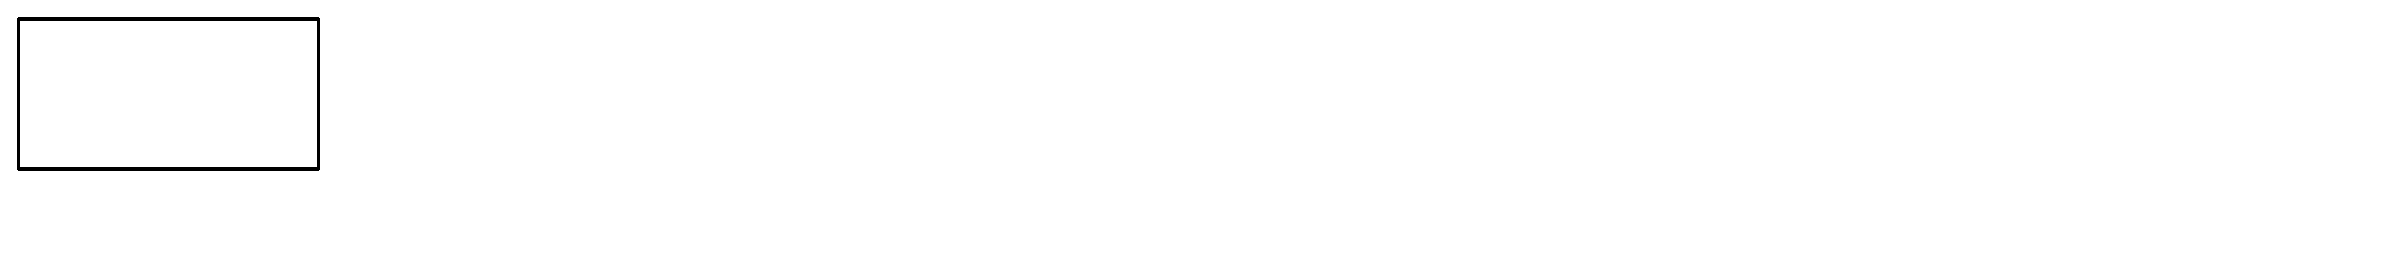
\includegraphics[width=1.05\textwidth]{figures/sort_join/empty_block.eps}};}
\onslide<2|handout:0>{\node at (0,0) {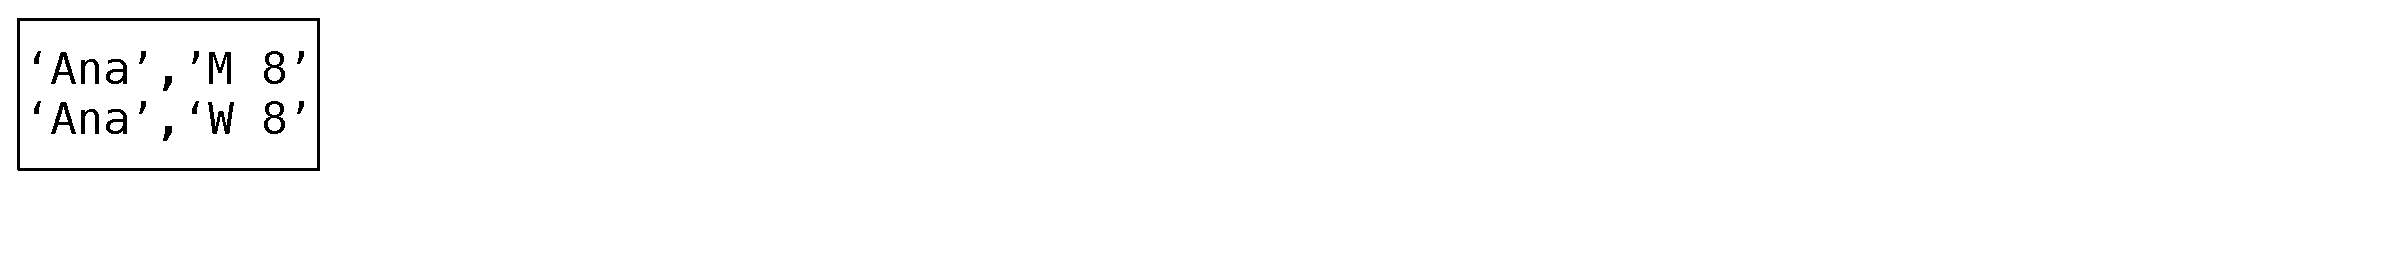
\includegraphics[width=1.05\textwidth]{figures/sort_join/step1.eps}};}
\onslide<3|handout:0>{\node at (0,0) {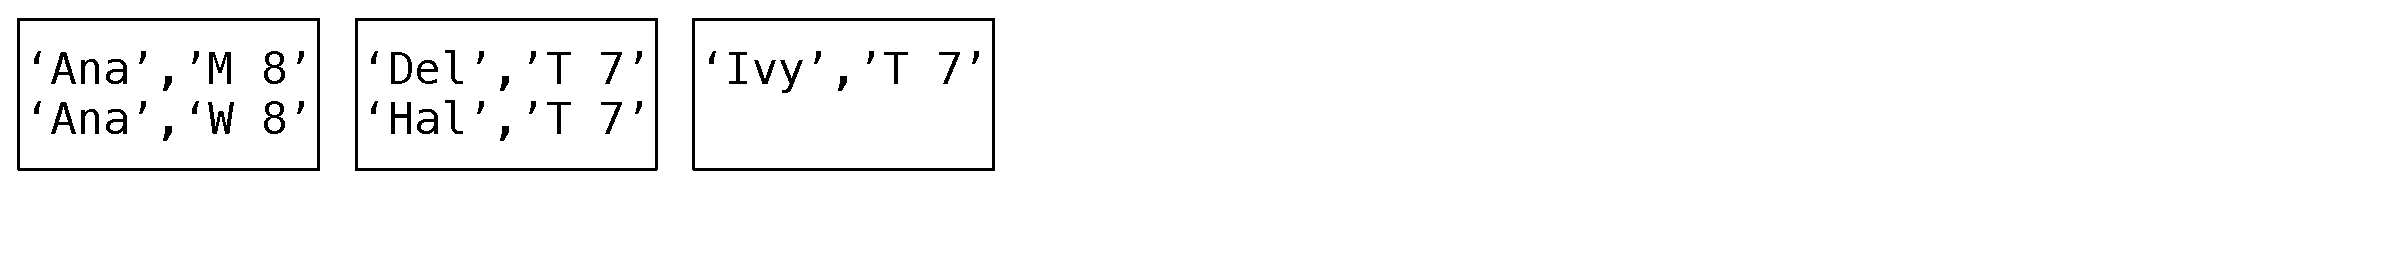
\includegraphics[width=1.05\textwidth]{figures/sort_join/step2.eps}};}
\onslide<4|handout:0>{\node at (0,0) {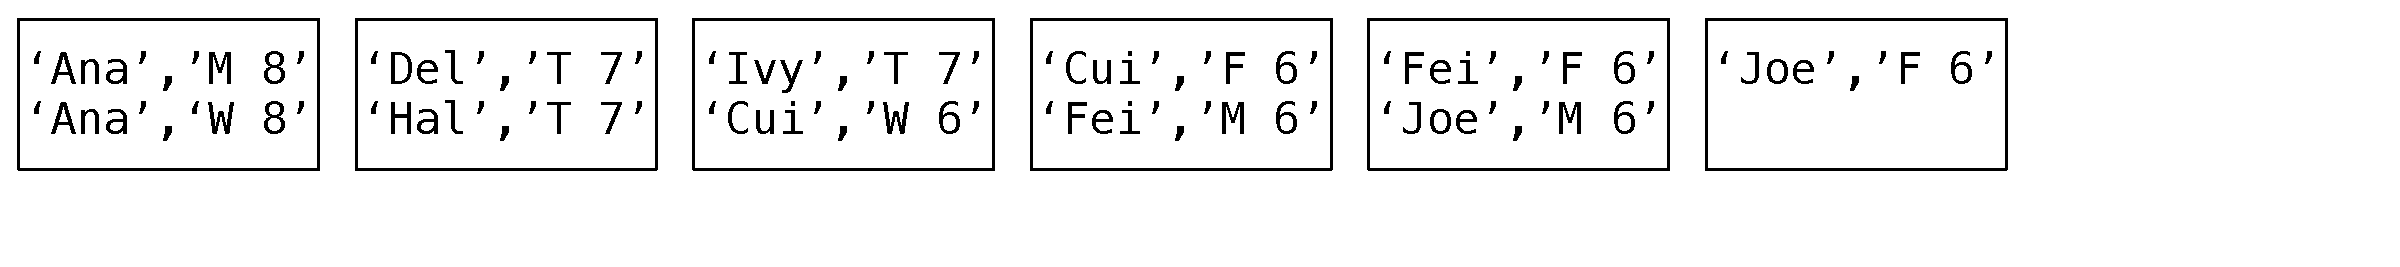
\includegraphics[width=1.05\textwidth]{figures/sort_join/step3.eps}};}
\onslide<6|handout:1>{\node at (0,0) {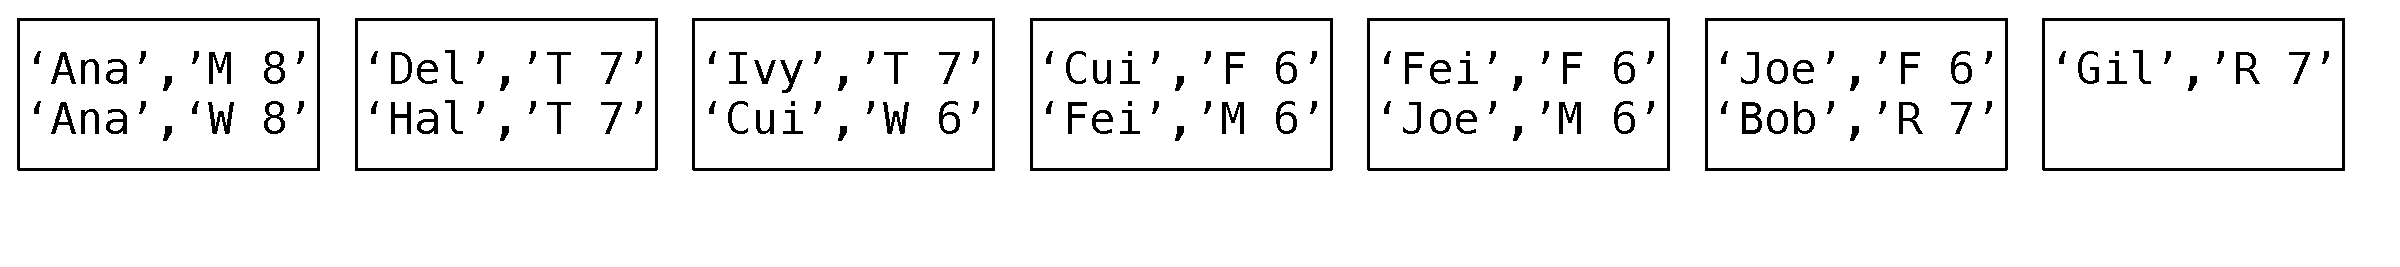
\includegraphics[width=1.05\textwidth]{figures/sort_join/step4.eps}};}
\end{tikzpicture}
\end{center}


\end{frame}


%
% --------------------------------------------------------------------------
%
\begin{frame}[fragile]
\label{sort_based_equality_join}

Pseudo-code of sort-based equality join. For simplicity, we refer to pointers to the tuples inside the sorted files.

\begin{center}
\scalebox{0.75}{\begin{minipage}{1.25\textwidth}%

\begin{algorithm}[H]
\begin{algorithmic}[1]
\caption*{\textbf{Open()} for sort-based evaluation of $R\Join_{R.a=S.b} S$}
\State $t_R \leftarrow $ first tuple in $R$; $t_{S1} \leftarrow $ first tuple in $S$; $t_{S2} \leftarrow t_{S1}$ 
\end{algorithmic}
\end{algorithm}
\end{minipage}}

\vskip0.75em

\scalebox{0.75}{\begin{minipage}{1.25\textwidth}%
\begin{algorithm}[H]
\begin{algorithmic}[1]
\caption*{\textbf{GetNext()} for sort-based evaluation of $R\Join_{R.a=S.b} S$}
	\While {$t_R.a \neq t_{S1}.b$} 
		\State \algorithmicif $t_R.a < t_{S1}.b$ 
			\algorithmicthen\  \alert{advance} $t_R$
			\algorithmicelse\  \alert{advance} $t_{S1}$ ; $t_{S2} = t_{S1}$
	\EndWhile
	\If {\lstinline[style=Python,mathescape]!$t_R = \ $ EOF!} \Comment {stop when there are no more tuples in $R$ to be joined}
		\State \Return \lstinline[style=Python,mathescape]!EOF!
	\EndIf
	\If {$t_R.a = t_{S2}.b$} 
		\State \lstinline[style=Python,mathescape]!$t \leftarrow$ join($t_R$, $t_{S2}$)!
		\State \alert{advance} $t_{S2}$
		\If {\lstinline[style=Python,mathescape]!$t_{S2} = \ $ EOF! \textbf{OR} 
		     \lstinline[style=Python,mathescape]!$t_{S2}.b > t_R.a$!} \Comment {all matches of the current $t_R$ found}
			\State \alert{advance} $t_R$ \Comment {the next call to \textbf{GetNext()} will find matches of the next $t_R$}
		\EndIf
		\State \lstinline[style=Python,mathescape]!yield $\ t$!
	\EndIf

\end{algorithmic}
\end{algorithm}
\end{minipage}}
\end{center}
\end{frame}

%
% --------------------------------------------------------------------------
%
\begin{frame}{Merge-Join on equality $R.a=S.b$}
\label{merge_join_algorithm}

If there are enough buffers to read all chunks of $R$ and $S$ concurrently, one can perform the join itself during the ``merge'' phase on the previous algorithm.

\textbf{Gist:} let $p$ point to the ``smallest'' tuple in $R$; find all matching tuples in $S$ (as in the previous algorithm); advance $p$; repeat.

\vskip1em

\begin{center}
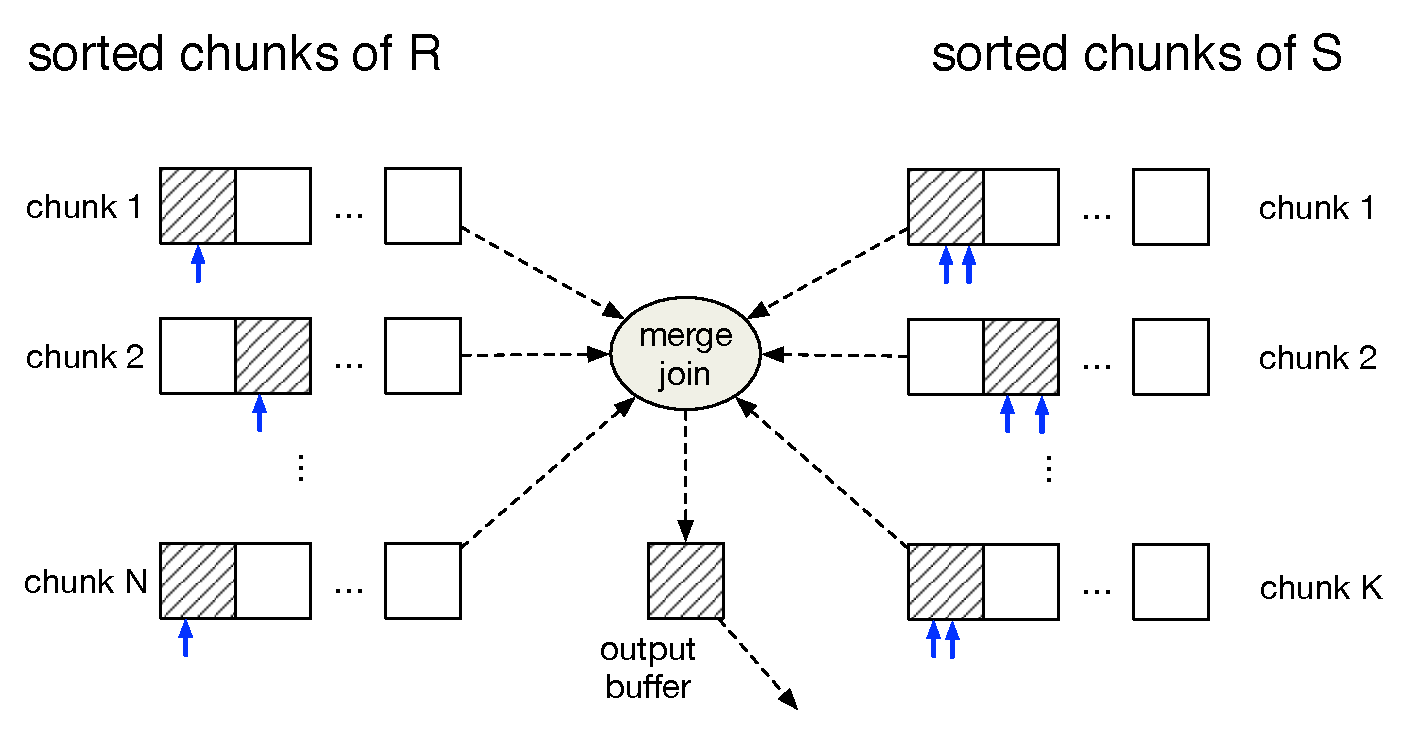
\includegraphics[width=0.75\textwidth]{figures/merge_join.pdf}
\end{center}
\end{frame}


%
% --------------------------------------------------------------------------
%
\begin{frame}
Example of merge-join:

\vskip2em

\begin{center}
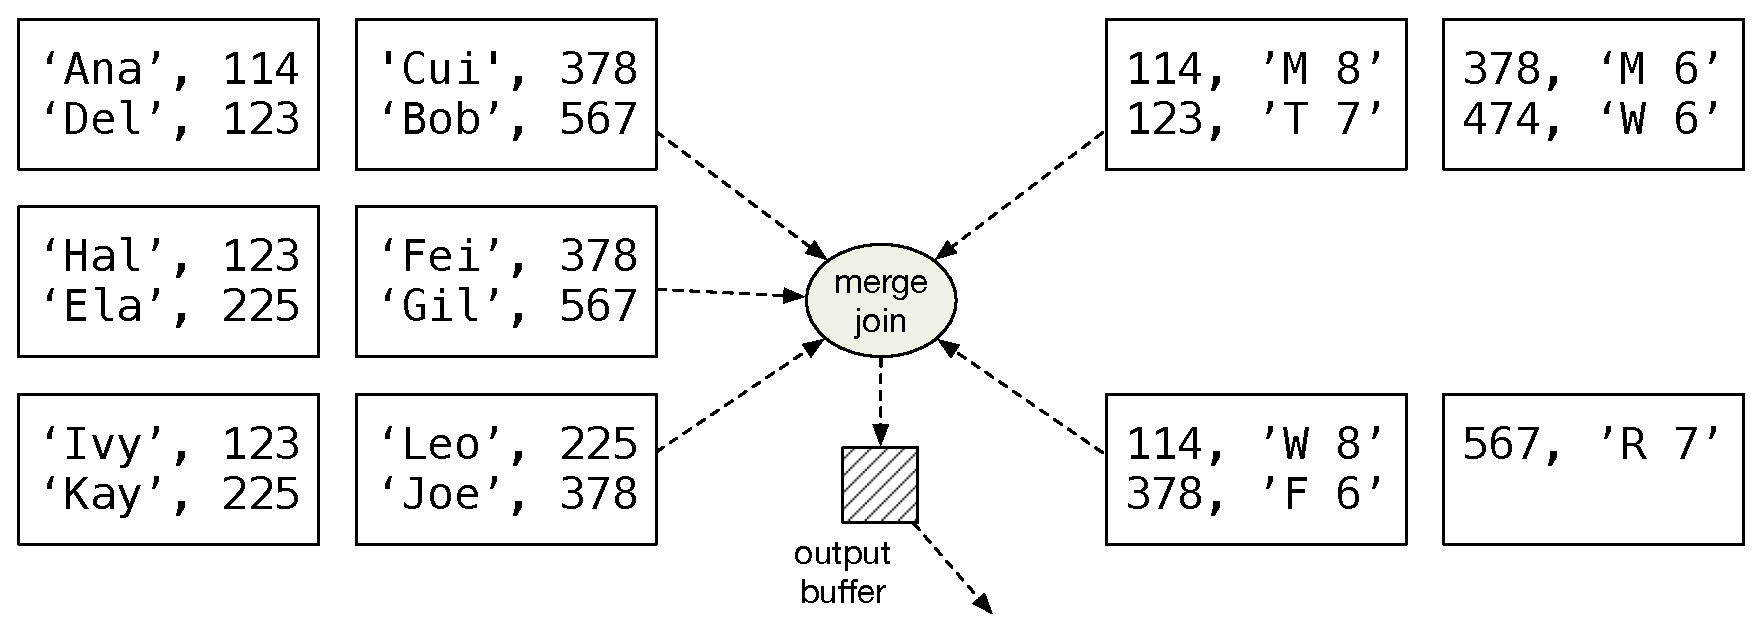
\includegraphics[width=0.9\textwidth]{figures/merge_join_example.eps}
\end{center}

\end{frame}

%
% --------------------------------------------------------------------------
%
\begin{frame}{Sort-based algorithms for other binary operators}
\label{generic_sort_merge_set_operator}

The same ``sort-merge'' framework can be used for the other binary operators.

\textbf{Set Union $R\cup S$}: copy the next ``smallest'' tuple amongst all pointers (in either $R$ and $S$) to the output; advance all pointers to duplicates of that tuple until they point to something else.

\begin{center}
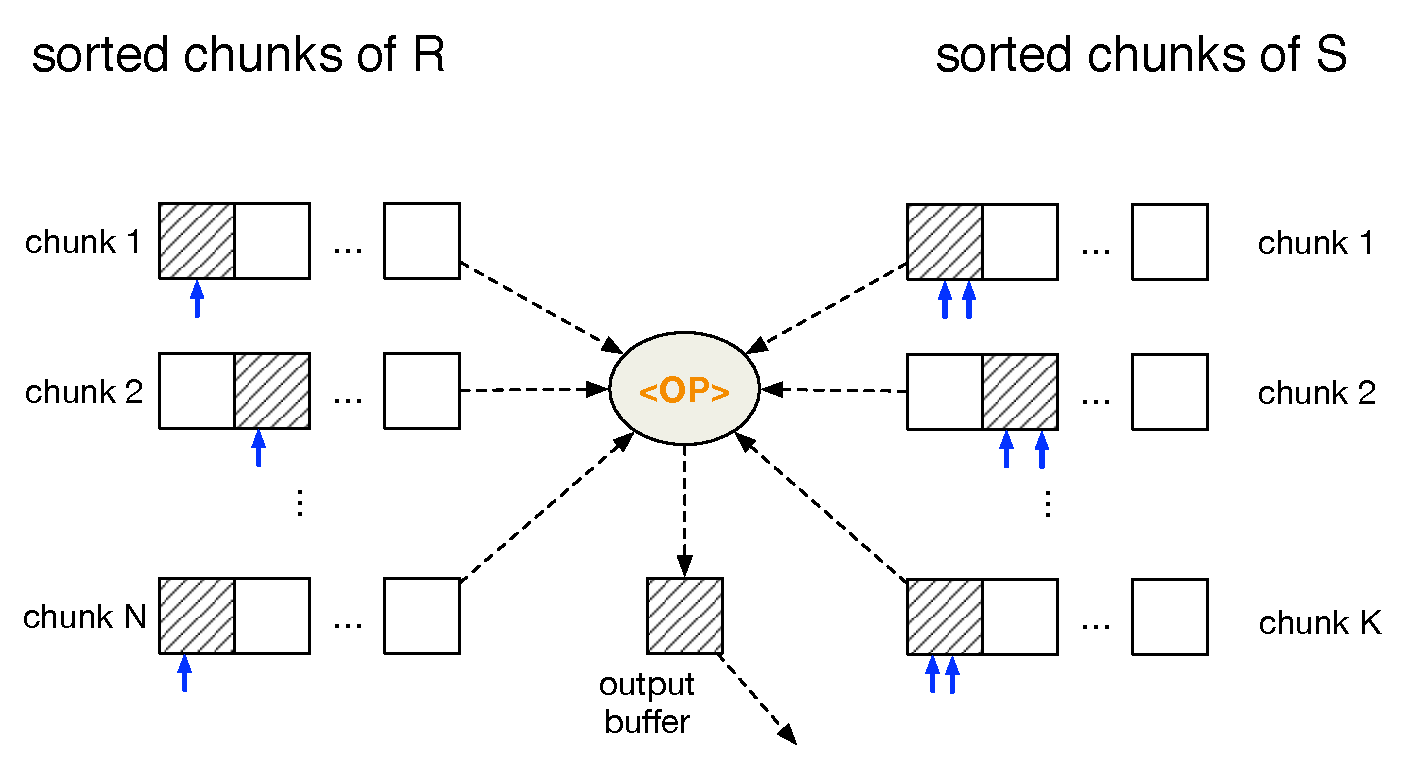
\includegraphics[width=0.75\textwidth]{figures/merge_OP.pdf}
\end{center}
\end{frame}


%
% --------------------------------------------------------------------------
%
\begin{frame}


\textbf{Set Intersection $R\cap S$}: copy the next ``smallest'' tuple that appears in both $R$ and $S$ to the output; advance all pointers to duplicates of that tuple until they point to something else.

\textbf{Set difference $R-S$}: copy the next ``smallest'' tuple in $R$ but not in $S$ (or vice-versa for $S-R$); advance all pointers on $R$ (or $S$, for $S-R$) until a new ``smallest'' tuple is found.

\begin{center}
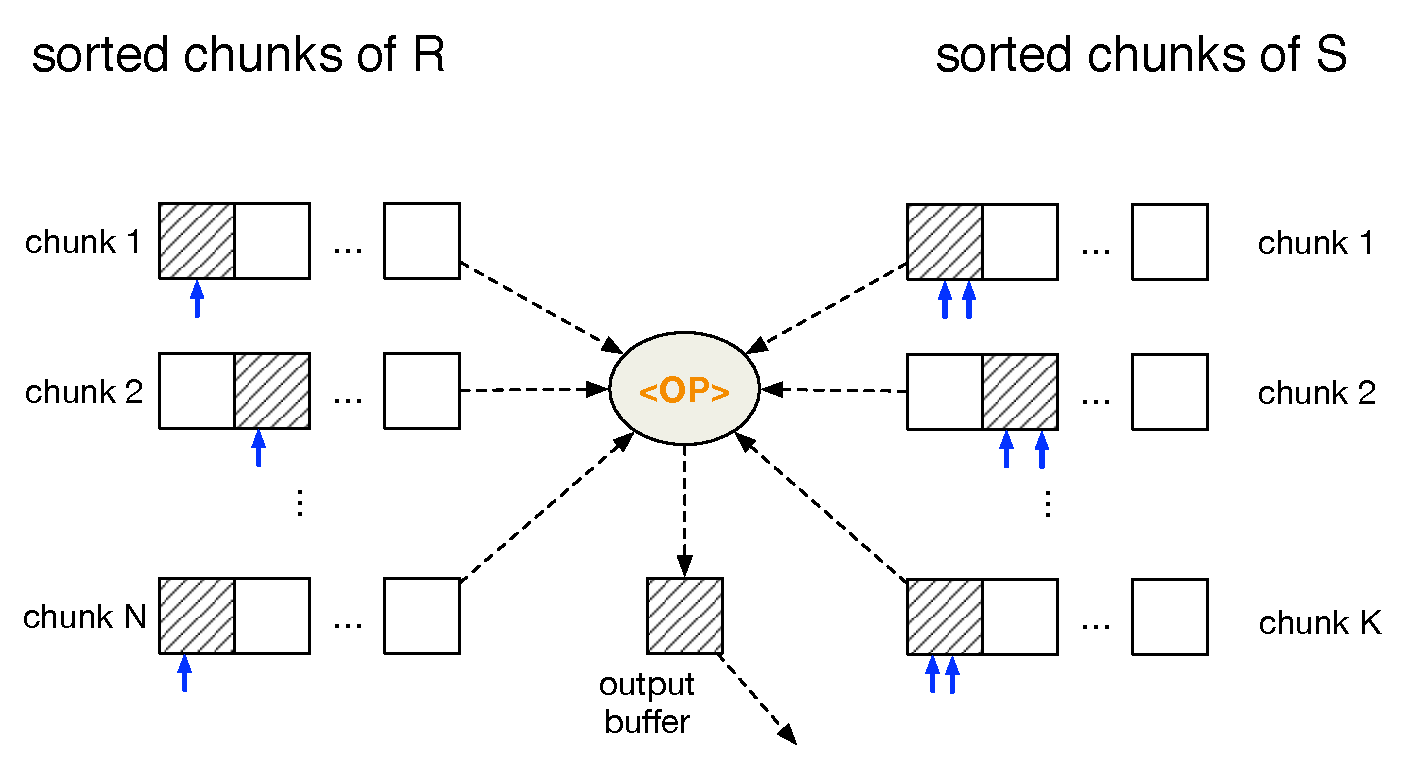
\includegraphics[width=0.75\textwidth]{figures/merge_OP.pdf}
\end{center}
\end{frame}